%%% CS6002 Project Report (AAMAS-style)
%%% No-Regret Learning in Stackelberg Security Games with an Unknown,
%%% Bounded Set of Attacker Types.
%%%
%%% Structure follows report_instructions.txt and visual format follows the
%%% AAMAS sigconf look of p597.pdf (two columns, tight margins, amsthm, natbib).

\documentclass[letterpaper,9pt,twocolumn]{extarticle}

\usepackage[top=0.85in,bottom=1in,left=0.7in,right=0.7in,columnsep=0.3in]{geometry}
\usepackage[utf8]{inputenc}
\usepackage[T1]{fontenc}
\usepackage{lmodern}
\usepackage{microtype}

\usepackage{amsmath,amssymb,amsthm}
\usepackage{mathtools}
\usepackage{bm}
\usepackage{graphicx}
\usepackage{booktabs}
\usepackage{algorithm}
\usepackage{algpseudocode}
\usepackage{enumitem}
\usepackage{xcolor}
\usepackage[hidelinks,breaklinks=true]{hyperref}
\usepackage[capitalise,noabbrev]{cleveref}
\usepackage[square,sort&compress,numbers]{natbib}
\bibliographystyle{abbrvnat}

% ---- Balcan et al. notation (Balcan, Blum, Haghtalab, Procaccia 2015) ----
\newcommand{\pvec}{\mathbf{p}}
\newcommand{\svec}{\mathbf{s}}
\newcommand{\avec}{\mathbf{a}}
\newcommand{\cP}{\mathcal{P}}
\newcommand{\cE}{\mathcal{E}}
\newcommand{\cD}{\mathcal{D}}
\newcommand{\cC}{\mathcal{C}}
\newcommand{\cM}{\mathcal{M}}
\newcommand{\EE}{\mathbb{E}}
\newcommand{\NN}{\mathbb{N}}
\newcommand{\RR}{\mathbb{R}}
\newcommand{\Kmax}{K_{\max}}
\newcommand{\Nmax}{N_{\max}}
\newcommand{\argmax}{\operatorname*{arg\,max}}
\newcommand{\argmin}{\operatorname*{arg\,min}}
\newcommand{\Regret}{\mathrm{Regret}}

% ---- Theorem environments ----
\theoremstyle{plain}
\newtheorem{theorem}{Theorem}
\newtheorem{lemma}[theorem]{Lemma}
\newtheorem{proposition}[theorem]{Proposition}
\newtheorem{corollary}[theorem]{Corollary}
\theoremstyle{definition}
\newtheorem{definition}[theorem]{Definition}
\newtheorem{problem}[theorem]{Problem}
\theoremstyle{remark}
\newtheorem{remark}[theorem]{Remark}

% ---- Header ----
\usepackage{fancyhdr}
\pagestyle{fancy}
\fancyhf{}
\renewcommand{\headrulewidth}{0pt}
\fancyfoot[C]{\thepage}

% ---- Title block ----
\title{\vspace{-2em}\textbf{\LARGE No-Regret Learning in Stackelberg Security Games\\
with an Unknown, Bounded Set of Attacker Types}}
\author{\normalsize
\begin{tabular}{ccc}
Aditi Singh & Ishita & Sabil Ahmad
\end{tabular}\\[0.2em]
\footnotesize\textit{Indian Institute of Technology Bombay}\\[0.1em]
\footnotesize CS\,6002 Project Report,  Spring 2026}
\date{\vspace{-1em}}

\begin{document}
\twocolumn[
  \begin{@twocolumnfalse}
  \maketitle
  % \begin{abstract}
% Stackelberg Security Games (SSGs) model the strategic allocation of limited
% defender resources against attackers whose preferences are often uncertain.
% \citet{balcan2015} designed no-regret online learning algorithms for the
% \emph{repeated} variant of SSGs against an adversarial sequence of attackers
% drawn from a finite, \emph{known} set $K$, and proved a matching linear-regret
% lower bound when $K$ is unbounded. A natural real-world middle ground is
% left open: the defender does not know $K$ a priori, but has a bound $\Kmax$
% on its size. We study this setting in the full-information feedback model.
% We propose \textsc{Grow-Catalogue}, an algorithm that incrementally learns
% new attacker types as they arrive, re-partitions the coverage polytope, and
% runs an anytime multiplicative-weights sub-routine on the resulting
% extreme-point set. Our central technical contribution is a full proof that
% \textsc{Grow-Catalogue} achieves expected regret
% \[
% O\!\left(\sqrt{T\cdot\Kmax\cdot(n^2+\Kmax\log n)}\right)
% \]
% against any oblivious adversarial sequence of length $T$. The rate matches
% that of \citet{balcan2015} with $k$ replaced by $\Kmax$ and is sublinear
% whenever $\Kmax\cdot(n^2+\Kmax\log n)=o(T)$. Experiments on synthetic SSG
% instances confirm the predicted $\sqrt{T}$ scaling, and the empirical regret
% stays comfortably below the analytic $C\sqrt{T}$ envelope. Code is available
% at \textcolor{blue}{\href{https://github.com/CS6002-SSG/grow-catalogue}{github.com/CS6002-SSG/grow-catalogue}}.
%   \end{abstract}
%   \vspace{0.6em}
  \end{@twocolumnfalse} 
]

% ==========================================================================

\section{Abstract}
\label{sec:Abstract}
Stackelberg Security Games (SSGs) model the strategic allocation of limited
defender resources against attackers whose preferences are often uncertain.
\citet{balcan2015} designed no-regret online learning algorithms for the
\emph{repeated} variant of SSGs against an adversarial sequence of attackers
drawn from a finite, \emph{known} set $K$, and proved a matching linear-regret
lower bound when $K$ is unbounded. A natural real-world middle ground is
left open: the defender does not know $K$ a priori, but has a bound $\Kmax$
on its size. We study this setting in the full-information feedback model.
We propose \textsc{Grow-Catalogue}, an algorithm that incrementally learns
new attacker types as they arrive, re-partitions the coverage polytope, and
runs an anytime multiplicative-weights sub-routine on the resulting
extreme-point set. Our central technical contribution is a full proof that
\textsc{Grow-Catalogue} achieves expected regret
\[
O\!\left(\sqrt{T\cdot\Kmax\cdot(n^2+\Kmax\log n)}\right)
\]
against any oblivious adversarial sequence of length $T$. The rate matches
that of \citet{balcan2015} with $k$ replaced by $\Kmax$ and is sublinear
whenever $\Kmax\cdot(n^2+\Kmax\log n)=o(T)$. Experiments on synthetic SSG
instances confirm the predicted $\sqrt{T}$ scaling, and the empirical regret
stays comfortably below the analytic $C\sqrt{T}$ envelope. Our implementation and all experiment scripts are at
\textcolor{blue}{\href{https://github.com/aditisingh1053/Security_Games}{github.com/aditisingh1053/Security\_Games}}.

\section{Introduction}
\label{sec:intro}

In a Stackelberg Security Game (SSG), a defender allocates a scarce set of
resources to protect $n$ potential targets against a strategic attacker
who, observing the defender's randomized deployment, chooses the best
target to attack \citep{tambe2012}. Deployed systems built around this model
include the US Coast Guard's port protection patrols, the Federal Air
Marshals assignment system, the LAX airport patrol schedule, and
anti-poaching patrols in several African national parks
\citep{tambe2012,yang2014}. In every one of these applications the
defender must commit to its deployment before the attack happens, and the
attacker's payoff function encodes its preferences over targets.

The \emph{classical} SSG analysis assumes that the attacker's payoff
function is fully known to the defender. The optimal commitment can then
be computed by a linear program \citep[e.g.,][]{pita2010}. In practice,
however, the defender faces considerable uncertainty about the attacker.
There may be several distinct threat actors (e.g., different poacher
groups, different types of smugglers), and their utilities are only
imperfectly known. A principled response, pioneered by \citet{balcan2015},
is to drop the single-type assumption entirely and instead ask for a
\emph{no-regret} online algorithm against an adversarially chosen sequence
of attacker types, drawn from a known finite set $K$ with $|K|=k$. Under
full-information feedback, they design an algorithm whose expected
cumulative regret is bounded by $O(\sqrt{Tn^2 k\log(nk)})$, which is
sublinear in the horizon $T$, and they prove a matching linear-regret lower
bound when $|K|$ is unrestricted \citep[Theorem~7.1]{balcan2015}.

The assumption that the set $K$ itself is known to the defender in advance
is, however, a strong one. In realistic deployments the defender typically
does \emph{not} have a complete list of attacker types at the start. What
it may have is an \emph{upper bound} $\Kmax$ on the number of distinct
types it expects to encounter (for instance, from threat intelligence or
from physical constraints of the domain). The question that motivates this
project is therefore:
\begin{center}
\emph{Can the defender achieve sublinear regret when $K$ is unknown a
priori, subject to $|K|\le \Kmax$?}
\end{center}
This question lies squarely in the gap left open between the
\emph{known-$K$} upper bound and the \emph{unrestricted-$K$} lower bound of
\citet{balcan2015}. It is not answered by any of the existing work, and
resolving it is the main goal of the present report.

\subsection{Contributions}
\label{sec:contrib}

Our contributions are the following.
\begin{itemize}[leftmargin=1.1em,itemsep=0.10em,topsep=0.2em]
  \item \textbf{Problem formalization (\Cref{sec:unknownK}).}
    We formalize the unknown-$K$ variant of the repeated Stackelberg
    security game, identifying the minimal modification of the model of
    \citet{balcan2015} that captures it.
  \item \textbf{Algorithm (\Cref{sec:alg}).}
    We propose \textsc{Grow-Catalogue}, an online algorithm that at each
    round maintains a \emph{catalogue} $C_t\subseteq K$ of attacker types
    observed so far, recomputes the set $\cE(C_t;\epsilon)$ of
    $\epsilon$-approximate extreme points of the partition of $\cP$
    induced by $C_t$, and runs an anytime multiplicative-weights
    sub-routine over $\cE(C_t)$. When a new type is observed, the
    catalogue is updated and the sub-routine is restarted on the enlarged
    expert set.
  \item \textbf{Main theorem and a complete, detailed proof
    (\Cref{sec:mainresult,sec:proof}).}
    The technical core of this report is a self-contained proof that
    \textsc{Grow-Catalogue} achieves expected regret at most
    $O(\sqrt{T\cdot\Kmax\cdot(n^2+\Kmax\log n)})$ against any oblivious
    adversarial sequence of length $T$ under full-information feedback.
    The rate matches Theorem~5.1 of \citet{balcan2015} with $k$ replaced
    by $\Kmax$; for constant $\Kmax$ it is $\tilde O(n\sqrt T)$.
  \item \textbf{Regime analysis (\Cref{cor:regime,cor:adaptive}).}
    We characterize the parameter regime in which the bound is meaningful
    ($\Kmax\cdot(n^2+\Kmax\log n)=o(T)$), and we prove an
    instance-adaptive refinement in which the leading factor depends on
    the number $K'$ of types \emph{actually} observed rather than on
    $\Kmax$.
  \item \textbf{Experiments (\Cref{sec:exp}).}
    We implement \textsc{Grow-Catalogue} and two reference baselines, and
    evaluate them on synthetic SSG instances. The empirical regret scales
    as predicted by the theorem, staying comfortably below the analytic
    $C\sqrt{T}$ envelope.
\end{itemize}

\subsection{Related Work}
\label{sec:related}

\paragraph{Classical SSGs and attacker uncertainty.}
The optimal commitment for a known attacker can be computed by an LP
\citep{conitzer2006}. Uncertainty about the attacker has been handled by
\emph{robust optimization}, which plans against worst-case payoffs
\citep{pita2010}, and by \emph{Bayesian SSGs}, which require a prior over
attacker types \citep{kiekintveld2011,marecki2012}. Both approaches rest on
priors or constraints that are often hard to validate. \citet{letchford2009}
give a query-efficient learning algorithm for a \emph{single} fixed but
unknown type, and \citet{blum2014b} extend this to a setting that adapts
round-by-round to one fixed type.

\paragraph{Online learning against adversarial attacker sequences.}
\citet{balcan2015} pivot from the single-type paradigm by allowing the
sequence of attackers to be adversarially chosen from a known finite set
$K$. For full information they give a polynomial-weights algorithm with
regret $O(\sqrt{Tn^2 k\log(nk)})$ that partitions the coverage polytope
into best-response regions and runs experts over the
$\epsilon$-approximate extreme points; for bandit feedback they use a
barycentric spanner construction to give an $O(T^{2/3})$ bound.
Crucially, they also prove a linear lower bound when $|K|$ is unrestricted,
which forces any non-trivial extension to restrict the attacker type set
somehow. We take the weakest restriction: a known cardinality bound
$\Kmax$.

\paragraph{Online learning with changing expert sets.}
The sub-routine inside \textsc{Grow-Catalogue} is an anytime variant of
Polynomial Weights / Hedge \citep{littlestone1994,freund1997,cesa2006}. We
restart this sub-routine each time the catalogue grows; simpler algorithms
for tracking a growing set of experts exist~\citep{mourtada2017}, and for
tracking a shrinking set \citep{gaillard2019}, but both would only shave
lower-order logarithmic factors.

\paragraph{Other recent directions.}
\citet{haghtalab2022} analyze no-regret learning against strategic
(non-myopic) attackers in a single-type query model. \citet{harris2024side}
extend to a contextual Stackelberg setting in which both players observe
side information. Neither addresses the \emph{unknown $K$ with bounded
cardinality} question that we pose here.
% ==========================================================================
\section{Model}
\label{sec:model}

We adopt the repeated-SSG notation of \citet[Sec.~2]{balcan2015}; our
notation is compatible with theirs.

\subsection{Game primitives}

The game has a finite horizon $T\in\NN$ and $n$ targets
$N=\{1,\dots,n\}$. The defender has $R$ resources and a collection
$\mathcal{D}\subseteq 2^N$ of \emph{schedules}, where each schedule is a
subset of targets that a single resource can defend simultaneously. An
\emph{assignment function} $A:R\to 2^{\mathcal{D}}$ records the schedules
that each resource may be assigned to. A \emph{pure strategy} is any valid
resource-to-schedule assignment; let $m$ denote the number of pure
strategies. A \emph{mixed strategy} is a distribution $\svec\in\Delta_m$
over pure strategies, and its induced \emph{coverage probability vector}
is $\pvec = M\svec\in [0,1]^n$, where $M\in\{0,1\}^{n\times m}$ has
$M_{ij}=1$ iff the $j$-th pure strategy covers target $i$. Write $\cP$ for
the set of valid coverage probability vectors;  Every coverage vector $\pvec$ is realizable by
some mixed strategy, and conversely every mixed strategy induces a unique
$\pvec\in\cP$.

\paragraph{Defender payoffs.}
For each target $i$, the defender has a payoff
$u_d^c(i)\in[-1,1]$ if $i$ is attacked \emph{and} covered, and a payoff
$u_d^u(i)\in[-1,1]$ if $i$ is attacked \emph{and uncovered}. The
defender's expected utility when target $i$ is attacked under coverage
$\pvec$ is therefore
\begin{equation}
U_d(i,\pvec)\;=\;u_d^c(i)\,p_i \;+\; u_d^u(i)\,(1-p_i),
\label{eq:Ud}
\end{equation}
which is \emph{linear} in $\pvec$ for each fixed target $i$.

\subsection{Attacker types and best response}

An attacker \emph{type} $\alpha$ is a pair
$(u_\alpha^c,u_\alpha^u)\in[-1,1]^n\times[-1,1]^n$ of per-target utilities
following the same ``covered/uncovered'' convention as the defender. Its
expected utility for attacking target $i$ under coverage $\pvec$ is
$
U_\alpha(i,\pvec)=u_\alpha^c(i)\,p_i + u_\alpha^u(i)\,(1-p_i).
$
Observing $\pvec$, type $\alpha$ \emph{best-responds}:
\begin{equation}
b_\alpha(\pvec)\;=\;\argmax_{i\in N}\,U_\alpha(i,\pvec),
\label{eq:br}
\end{equation}
with ties broken arbitrarily but consistently. Note that $b_\alpha$ is
piecewise constant in $\pvec$, which makes the defender's realized payoff
$U_d(b_\alpha(\pvec),\pvec)$ a discontinuous function of $\pvec$. This
non-continuity is the central technical difficulty that distinguishes SSGs
from vanilla online linear optimization, and it is what drives the
polytope-based machinery of \citet{balcan2015}.

\subsection{Repeated game and regret}

There is a (possibly unknown) set $K$ of attacker types. An
\emph{oblivious} adversary chooses a sequence
$\avec=a_1,\dots,a_T\in K^T$ \emph{before} the game starts; the sequence
is fixed but unknown to the defender. At each round
$t\in\{1,\dots,T\}$ the defender commits $\pvec_t\in\cP$, attacker
$a_t$ plays $b_{a_t}(\pvec_t)$, and the defender receives the random
payoff $U_d(b_{a_t}(\pvec_t),\pvec_t)$. We assume \emph{full-information
feedback}: at the end of round $t$ the defender observes the identity of
$a_t$, and the first time any type $\alpha$ is observed, its utility
functions are revealed as well.

The defender's benchmark is the best fixed coverage vector in hindsight:
\begin{equation}
\pvec^{*}\;=\;\argmax_{\pvec\in\cP}\;\sum_{t=1}^T U_d\bigl(b_{a_t}(\pvec),\pvec\bigr).
\label{eq:pstar}
\end{equation}
The expected regret of an online algorithm that plays $\pvec_t$ at round
$t$ is
\begin{equation}
\Regret(T)\;=\;\sum_{t=1}^T\!U_d(b_{a_t}(\pvec^{*}),\pvec^{*})\;-\;\EE\!\bigg[\sum_{t=1}^T\!U_d(b_{a_t}(\pvec_t),\pvec_t)\bigg],
\label{eq:regret}
\end{equation}
where the expectation is over the algorithm's internal randomization.

\subsection{Preliminaries: polytope partition and $\cE(C;\epsilon)$}
\label{sec:polytopes}

The following definitions, taken from \citet[Sec.~4]{balcan2015}, are
essential. For any catalogue $C\subseteq K$, a type $\alpha\in C$, and a
target $i\in N$, the region in which $\alpha$'s best response is $i$ is
\begin{equation}
\cP^\alpha_i(C)\;=\;\{\pvec\in\cP\,:\,b_\alpha(\pvec)=i\},
\label{eq:Pia}
\end{equation}
which is the intersection of $\cP$ with the $n-1$ linear inequalities
$U_\alpha(i,\pvec)\ge U_\alpha(j,\pvec)$ for $j\ne i$; hence a convex
polytope. For a \emph{response profile}
$\sigma:C\to N$ we write
\begin{equation}
\cP_\sigma(C)\;=\;\bigcap_{\alpha\in C}\cP^\alpha_{\sigma(\alpha)}(C).
\label{eq:Psigma}
\end{equation}
The non-empty sets $\cP_\sigma(C)$ form a partition of $\cP$ into convex
regions in which the best response of every type in $C$ is held fixed;
within any such region, the defender's payoff under a fixed attacker type
is a linear function of $\pvec$.

We will need three results from \citet{balcan2015}, restated below in our
notation and cited explicitly at every use. \Cref{lem:43,lem:44} describe
the approximate extreme-point set; \Cref{prop:hedge} is the standard
Polynomial-Weights online learning guarantee, adapted to the present loss
range.

\begin{lemma}[{\citealp[Lemma 4.3]{balcan2015}}]
\label{lem:43}
For every $\epsilon>0$ and every catalogue $C\subseteq K$, there is a
finite set $\cE(C;\epsilon)\subseteq \cP$ of points, called the
$\epsilon$-approximate extreme points of the partition, such that for any
sequence $\avec'=a'_1,\dots,a'_{T'}$ with $a'_t\in C$ for all $t$,
\[
\max_{\pvec\in\cE(C;\epsilon)}\!\sum_{t=1}^{T'}\!U_d(b_{a'_t}(\pvec),\pvec)\,\ge\,\max_{\pvec\in\cP}\!\sum_{t=1}^{T'}\!U_d(b_{a'_t}(\pvec),\pvec)-2\epsilon\,T'.
\]
\end{lemma}

\begin{lemma}[{\citealp[Lemma 4.4]{balcan2015}}]
\label{lem:44}
The set $\cE(C;\epsilon)$ of \Cref{lem:43} can be chosen so that
\(|\cE(C;\epsilon)|\in O\!\bigl((2^n+|C|\,n^2)^n\cdot n^{|C|}\bigr).\)
\end{lemma}

\begin{proposition}[{\citealp[Proposition 1]{balcan2015}}]
\label{prop:hedge}
For any fixed expert set $\cM$ and any sequence of losses in
$[-\kappa,\kappa]$, there is an online learning algorithm (an anytime
variant of Polynomial Weights / Hedge; see \citealp[Sec.~2]{cesa2006}) whose
expected regret after $T'$ rounds is at most
$O\bigl(\sqrt{T'\,\kappa\,\log|\cM|}\bigr)$, without requiring $T'$ to be
known in advance.
\end{proposition}

% ==========================================================================
\section{The Unknown-$K$ Setting}
\label{sec:unknownK}

We now state the problem that our algorithm and theorem address.

\begin{problem}[Unknown-$K$ repeated SSG]\label{prob:unknownK}
A repeated SSG as in \Cref{sec:model} is played, with two modifications.
\begin{enumerate}[leftmargin=1.2em,itemsep=0.05em,topsep=0.2em]
  \item The set $K$ of attacker types is not revealed to the defender at
  the start; however, the defender is given a constant $\Kmax\ge 1$ with
  the promise $|K|\le\Kmax$.
  \item Feedback is full information: after round $t$ the defender
  observes $a_t$, and the first time any type $\alpha$ appears, its
  utility vectors $(u_\alpha^c,u_\alpha^u)$ are revealed.
\end{enumerate}
The benchmark $\pvec^{*}$ and regret $\Regret(T)$ are as in
\Cref{eq:pstar,eq:regret}.
\end{problem}

\begin{remark}[Necessity of the bound $\Kmax$]\label{rem:necessity}
\citet[Theorem 7.1]{balcan2015} exhibit, for every $T$, a game with
$|K|<2^{T+1}$ on which every online algorithm has expected regret at
least $T/2$. Hence some finite bound on $|K|$ is \emph{necessary} for
sublinear regret; \Cref{prob:unknownK} takes the weakest such bound,
namely a known constant $\Kmax$.
\end{remark}



% ==========================================================================
\section{Algorithm and Main Result}
\label{sec:alg}

\subsection{The \textsc{Grow-Catalogue} algorithm}

We describe \textsc{Grow-Catalogue} at a high level and then give the
pseudocode in \Cref{alg:gc}. At any round $t$ the defender holds a
catalogue $C_t\subseteq K$ of all types seen so far. Conceptually, the
defender runs a small instance of the \emph{known-$K$} algorithm of
\citet[Sec.~5]{balcan2015} on the catalogue $C_t$, pretending that $C_t$
\emph{is} the full attacker set. Concretely:
\begin{itemize}[leftmargin=1.1em,itemsep=0.05em,topsep=0.2em]
  \item The algorithm maintains the $\epsilon$-approximate extreme-point
  set $\cE_t=\cE(C_t;\epsilon)$ of \Cref{lem:43}. We set
  $\epsilon=1/\sqrt T$; this balances the $2\epsilon T$ approximation term
  in \Cref{lem:43} against the $\sqrt{T\log\Nmax}$ regret term of
  \Cref{prop:hedge}.
  \item An anytime Polynomial-Weights sub-routine of
  \Cref{prop:hedge} runs over $\cE_t$, updating via a time-varying
  learning rate $\eta_{t_{\text{loc}}}=\sqrt{\log|\cE_t|/t_{\text{loc}}}$
  where $t_{\text{loc}}$ is a local counter reset at every catalogue
  change. This is the standard anytime schedule; see \citet[Sec.~2]{cesa2006}.
  \item When a new attacker type $\alpha$ appears, the catalogue grows to
  $C_t\cup\{\alpha\}$, the approximate extreme-point set is recomputed,
  and the sub-routine is restarted on the enlarged expert set. The single
  round of first contact with $\alpha$ contributes a bounded additive
  amount to the regret that we will absorb.
\end{itemize}

\begin{algorithm}[t]
\caption{\textsc{Grow-Catalogue} (full information).}
\label{alg:gc}
\begin{algorithmic}[1]
\small
\Require horizon $T$, bound $\Kmax$, game primitives, default $\pvec_{\text{def}}\in\cP$
\State $C\gets\emptyset$;~$\cE\gets\emptyset$;~$\epsilon\gets 1/\sqrt T$;~$t_{\text{loc}}\gets 0$
\For{$t=1,\dots,T$}
  \If{$\cE=\emptyset$} \State play $\pvec_t\gets\pvec_{\text{def}}$
  \Else \State sample $\pvec_t\sim q_t$, where $q_t$ is the current PW distribution over $\cE$
  \EndIf
  \State observe $a_t$
  \If{$a_t\notin C$} \Comment{discovery round: new attacker type}
    \State $C\gets C\cup\{a_t\}$; record $(u_{a_t}^c,u_{a_t}^u)$
    \State $\cE\gets\cE(C;\epsilon)$ \Comment{recompute extreme points}
    \State reset PW on $\cE$; $t_{\text{loc}}\gets 0$
  \Else \Comment{routine round}
    \State $t_{\text{loc}}\gets t_{\text{loc}}+1$
    \State compute $\ell_t(\pvec)\!=\!-U_d(b_{a_t}(\pvec),\pvec)$ for $\pvec\in\cE$
    \State $\eta\gets\sqrt{\log|\cE|/t_{\text{loc}}}$
    \State $w_\pvec\gets w_\pvec\cdot e^{-\eta\,\ell_t(\pvec)}$ for all $\pvec\in\cE$
  \EndIf
\EndFor
\end{algorithmic}
\end{algorithm}


\subsection{Main Result}
\label{sec:mainresult}

\begin{theorem}[Main]
\label{thm:main}
Let the defender play \Cref{alg:gc} in the unknown-$K$ full-information
setting of \Cref{prob:unknownK}. For any oblivious adversarial sequence
$\avec\in K^T$ with $|K|\le\Kmax$, the expected regret satisfies
\begin{equation}
\EE[\Regret(T)]\;\le\;O\!\Bigl(\sqrt{T\cdot\Kmax\cdot(n^2+\Kmax\log n)}\Bigr).
\label{eq:main}
\end{equation}
In particular, if $\Kmax=O(1)$ then $\EE[\Regret(T)]=\tilde O(n\sqrt T)$,
matching the known-$K$ bound of \citet[Theorem 5.1]{balcan2015} up to
logarithmic factors.
\end{theorem}

We prove \Cref{thm:main} in detail in \Cref{sec:proof}. Two useful
corollaries of the proof (the regime of applicability and an
instance-adaptive refinement) are stated after the proof in
\Cref{sec:consequences}.

% ==========================================================================
\section{Proof of \Cref{thm:main}}
\label{sec:proof}

The proof closely tracks the structure of the known-$K$ proof of \citet[Sec.~5]{balcan2015}
but has two non-trivial deviations: (i) the expert set is no longer static
but grows over time, and (ii) the discovery rounds introduce an extra
bounded additive term. We account for both the deviations in our proof.

\begin{proof}[Proof:- ]
Fix an oblivious adversarial sequence $\avec=a_1,\dots,a_T\in K^T$ with
$|K|\le\Kmax$. Let $K'=|\{a_1,\dots,a_T\}|\le\Kmax$ denote the number of
distinct types that actually appear in $\avec$. The proof proceeds in ten
steps.

\paragraph{Step 1 (Epoch decomposition).}
Let $\tau_1<\tau_2<\cdots<\tau_{K'}$ be the round indices at which each
new attacker type is first observed, i.e., for each
$i\in\{1,\dots,K'\}$, round $\tau_i$ is the smallest $t$ such that
$a_t\notin\{a_1,\dots,a_{t-1}\}$. We define the \emph{epochs}
\begin{equation}
\mathrm{Ep}_i\;=\;\{\tau_i+1,\tau_i+2,\dots,\tau_{i+1}-1\},\quad
i=1,\dots,K',
\label{eq:epoch-def}
\end{equation}
with the convention $\tau_{K'+1}\coloneqq T+1$, and write
$L_i=|\mathrm{Ep}_i|$. Let
$\mathcal{D}=\{\tau_1,\dots,\tau_{K'}\}$ be the set of \emph{discovery
rounds}. By construction,
\[
[1,T]\;=\;\mathcal{D}\;\sqcup\;\bigcup_{i=1}^{K'}\mathrm{Ep}_i,
\]
and
$|\mathcal{D}|+\sum_{i=1}^{K'}L_i=T$ with $|\mathcal{D}|=K'\le\Kmax$. The
epoch decomposition is the critical structural property of the proof: it
re-interprets the online problem with a growing expert set as a finite
sequence of online problems with \emph{fixed} expert sets, so that the
known-$K$ analysis of \citet{balcan2015} can be invoked inside each
epoch.

\paragraph{Step 2 (Catalogue is constant inside an epoch).}
Immediately after round $\tau_i$, the catalogue maintained by
\Cref{alg:gc} is $C_i=\{a_{\tau_1},\dots,a_{\tau_i}\}$, and it is not
updated until the next discovery round $\tau_{i+1}$. Hence $C_t=C_i$ for
every $t\in\mathrm{Ep}_i$. Moreover, by the defining property of
$\tau_{i+1}$, no new type appears in $\mathrm{Ep}_i$, so
\begin{equation}
a_t\in C_i\quad\text{for every }t\in\mathrm{Ep}_i.
\label{eq:epoch-types}
\end{equation}
Denote by $\cE_i\coloneqq\cE(C_i;\epsilon)$ the extreme-point set
used by the PW sub-routine during $\mathrm{Ep}_i$; \Cref{eq:epoch-types}
is exactly the hypothesis needed to apply \Cref{lem:43} to $C_i$ and the
sub-sequence inside $\mathrm{Ep}_i$.

\paragraph{Step 3 (Within-epoch regret).}
During $\mathrm{Ep}_i$ the algorithm runs a fresh instance of the anytime
Polynomial-Weights sub-routine on the fixed expert set $\cE_i$ for $L_i$
rounds. The losses are $\ell_t(\pvec)=-U_d(b_{a_t}(\pvec),\pvec)\in[-1,1]$,
so the range parameter is $\kappa=1$. \Cref{prop:hedge} therefore
yields an absolute constant $c_1>0$ such that
\begin{align}
&\max_{\pvec\in\cE_i}\sum_{t\in\mathrm{Ep}_i}\!U_d(b_{a_t}(\pvec),\pvec)\notag\\
&\quad-\EE\!\left[\sum_{t\in\mathrm{Ep}_i}\!U_d(b_{a_t}(\pvec_t),\pvec_t)\right]\;\le\;c_1\sqrt{L_i\log|\cE_i|}.
\label{eq:hedge-epoch}
\end{align}

\paragraph{Step 4 (Within-epoch approximation via \Cref{lem:43}).}
We now wish to compare the max over $\cE_i$ during $\mathrm{Ep}_i$ with
the \emph{global} benchmark $\pvec^{*}$ (the best fixed strategy over the
full horizon $[1,T]$). \Cref{lem:43}, however, is a statement of the form
``$\max_{\pvec\in\cE(C;\epsilon)}(\cdot)\ge\max_{\pvec\in\cP}(\cdot)-2\epsilon T'$''
and, strictly speaking, does \emph{not} directly involve $\pvec^{*}$: it
compares the max over the finite set $\cE(C;\epsilon)$ against the
unrestricted max over $\cP$, both on the \emph{same} attacker sequence.
We therefore proceed in two sub-steps and make the passage to $\pvec^{*}$
explicit.

\emph{Sub-step 4a (apply \Cref{lem:43} to the epoch sub-sequence).}
By \Cref{eq:epoch-types}, the sub-sequence $(a_t)_{t\in\mathrm{Ep}_i}$
has length $L_i$ and uses only types in $C_i$, which is exactly the
hypothesis of \Cref{lem:43}. Applying the lemma with catalogue $C_i$ and
sequence length $T'=L_i$ gives
\begin{align}
&\max_{\pvec\in\cE_i}\!\sum_{t\in\mathrm{Ep}_i}\!U_d(b_{a_t}(\pvec),\pvec)\notag\\
&\quad\ge\;\underbrace{\max_{\pvec\in\cP}\!\sum_{t\in\mathrm{Ep}_i}\!U_d(b_{a_t}(\pvec),\pvec)}_{\eqqcolon\;\mathrm{OPT}_i}-2\epsilon L_i.
\label{eq:lem43-epoch}
\end{align}
Here $\mathrm{OPT}_i$ is the best cumulative utility achievable on
$\mathrm{Ep}_i$ by \emph{any} coverage vector in $\cP$; crucially, this
is the epoch-$i$ optimum, which in general \emph{differs} from the value
of $\pvec^{*}$. This is the subtle point that distinguishes
our setting from the known-$K$ proof of \citet[Sec.~5]{balcan2015}: in their
analysis, \Cref{lem:43} is applied once on the full horizon, so
$\mathrm{OPT}=\sum_{t=1}^T U_d(b_{a_t}(\pvec^{*}),\pvec^{*})$ by
definition of $\pvec^{*}$ and no separate passage is needed. In our
per-epoch application, $\mathrm{OPT}_i$ is an epoch-local quantity,
potentially larger than $\pvec^{*}$'s value on the epoch.

\emph{Sub-step 4b (pass from $\mathrm{OPT}_i$ to $\pvec^{*}$).}
Since $\pvec^{*}\in\cP$, the coverage vector $\pvec^{*}$ is a \emph{feasible}
competitor in the maximization defining $\mathrm{OPT}_i$. Therefore
\begin{equation}
\mathrm{OPT}_i\;\ge\;\sum_{t\in\mathrm{Ep}_i}\!U_d(b_{a_t}(\pvec^{*}),\pvec^{*}).
\label{eq:opt-vs-pstar}
\end{equation}
Inequality \Cref{eq:opt-vs-pstar} is \emph{not} a consequence of
\Cref{lem:43} but of the trivial fact that the global benchmark
$\pvec^{*}$ is an element of the set over which the epoch-local optimum
is taken. Chaining \Cref{eq:lem43-epoch} with \Cref{eq:opt-vs-pstar},
\begin{align}
&\max_{\pvec\in\cE_i}\!\sum_{t\in\mathrm{Ep}_i}\!U_d(b_{a_t}(\pvec),\pvec)\notag\\
&\quad\ge\;\sum_{t\in\mathrm{Ep}_i}\!U_d(b_{a_t}(\pvec^{*}),\pvec^{*})-2\epsilon L_i.
\label{eq:lem43-pstar}
\end{align}


\paragraph{Step 5 (Per-epoch combined bound).}
Chaining \Cref{eq:hedge-epoch,eq:lem43-pstar}, for every epoch
$i\in\{1,\dots,K'\}$ we obtain
\begin{align}
&\EE\!\left[\sum_{t\in\mathrm{Ep}_i}\!U_d(b_{a_t}(\pvec_t),\pvec_t)\right]\notag\\
&\;\ge\;\sum_{t\in\mathrm{Ep}_i}\!U_d(b_{a_t}(\pvec^{*}),\pvec^{*})-2\epsilon L_i-c_1\sqrt{L_i\log|\cE_i|}.\label{eq:combined-epoch}
\end{align}
Equation \Cref{eq:combined-epoch} is the per-epoch regret bound
\emph{against the global benchmark} $\pvec^{*}$, and it is the building
block for the rest of the proof. Note that despite the fact that
$\pvec^{*}$ is the benchmark over all $T$ rounds (not just epoch $i$),
we are able to bound our per-epoch regret against $\pvec^{*}$ because
$\pvec^{*}\in\cP$ and we applied \Cref{lem:43} on the sub-sequence.

\paragraph{Step 6 (Discovery rounds).}
For each discovery round $t\in\mathcal{D}$, the algorithm either plays
$\pvec_{\text{def}}$ (if $t=\tau_1$) or samples $\pvec_t$ from the PW
distribution inherited from $\mathrm{Ep}_{i-1}$ (if $t=\tau_i$ for
$i\ge 2$). In both cases the sampled $\pvec_t$ is not tuned to the
newly-appearing type $a_t=a_{\tau_i}$. However, because the payoff
$U_d$ is bounded in $[-1,1]$, for every $\pvec\in\cP$ and every type
$\alpha$, $U_d(b_\alpha(\pvec),\pvec)\in[-1,1]$, so
\begin{equation}
\bigl|U_d(b_{a_t}(\pvec^{*}),\pvec^{*})-U_d(b_{a_t}(\pvec_t),\pvec_t)\bigr|\;\le\;2.
\label{eq:disc-bound}
\end{equation}
Summing \Cref{eq:disc-bound} over the at most $K'\le\Kmax$ discovery rounds
yields
\begin{equation}
\sum_{t\in\mathcal{D}}\!U_d(b_{a_t}(\pvec^{*}),\pvec^{*})-\EE\!\left[\sum_{t\in\mathcal{D}}\!U_d(b_{a_t}(\pvec_t),\pvec_t)\right]\le 2\Kmax.
\label{eq:disc-sum}
\end{equation}
This is the only source of additive dependence on $\Kmax$ that does not
come from the main $\sqrt{T\Kmax}$ term. It is the ``price of not knowing
$K$'' at a discovery round.

\paragraph{Step 7 (Uniform bound on $|\cE_i|$).}
By \Cref{lem:44} applied with $|C_i|\le\Kmax$,
\[
|\cE_i|\;\le\;c_2\,(2^n+\Kmax n^2)^n\cdot n^{\Kmax}\;\eqqcolon\;\Nmax,
\]
for an absolute constant $c_2$. Taking logarithms,
\begin{align}
\log\Nmax &= n\log\!\bigl(2^n+\Kmax n^2\bigr)+\Kmax\log n+O(1)\notag\\
&\le n^2+n\log\!\bigl(1+\tfrac{\Kmax n^2}{2^{n-1}}\bigr)+\Kmax\log n\notag\\
&= O\bigl(n^2+\Kmax\log n\bigr),
\label{eq:logN}
\end{align}
where the middle step uses $\log(2^n+\Kmax n^2)\le n+\log(1+\Kmax n^2/2^{n-1})$
and $\log(1+x)\le x$ for $x>0$. Crucially, \Cref{eq:logN} is uniform in
$i$: $\log|\cE_i|\le\log\Nmax$ for every epoch. This lets us pull the
$\log|\cE_i|$ factor in Step~5 outside the sum over epochs.

\paragraph{Step 8 (Summing across epochs).}
Sum \Cref{eq:combined-epoch} over $i=1,\dots,K'$ and add
\Cref{eq:disc-sum}. The algorithm's total expected utility is then at
least the benchmark's total utility, minus the discovery term $2\Kmax$,
minus $2\epsilon T$ from the telescoping Lemma-4.3 approximation errors
(using $\sum_i L_i\le T$), minus the sum of the per-epoch PW regret
terms. Rearranging,
\begin{align}
\EE[\Regret(T)]\;\le\;2\Kmax+2\epsilon T+c_1\sqrt{\log\Nmax}\!\sum_{i=1}^{K'}\!\sqrt{L_i}.
\label{eq:after-sum}
\end{align}

\paragraph{Step 9 (Cauchy--Schwarz).}
The last term involves the sum of $K'$ square roots. By the Cauchy--Schwarz
inequality applied to $(1,\dots,1)\in\RR^{K'}$ and
$(\sqrt{L_1},\dots,\sqrt{L_{K'}})$,
\begin{equation}
\sum_{i=1}^{K'}\!\sqrt{L_i}\;\le\;\sqrt{K'\cdot\!\sum_{i=1}^{K'}\!L_i}\;\le\;\sqrt{\Kmax\,T}.
\label{eq:CS}
\end{equation}
The first inequality is tight when all epochs have equal length, a
scenario that corresponds to an adversary who reveals types evenly across
the horizon. This is where the leading multiplicative $\sqrt{\Kmax}$
factor in the bound is generated. An instance-adaptive version uses $K'$
in place of $\Kmax$, which is what \Cref{cor:adaptive} records.

\paragraph{Step 10 (Final substitution).}
Plugging \Cref{eq:logN,eq:CS} into \Cref{eq:after-sum} and choosing
$\epsilon=1/\sqrt T$ gives
\begin{align*}
\EE[\Regret(T)]&\le 2\Kmax+2\sqrt T+c_1\sqrt{\Kmax T\,\log\Nmax}\\
&\le 2\Kmax+2\sqrt T\\
&\quad+c_3\sqrt{T\Kmax(n^2+\Kmax\log n)}
\end{align*}
for an absolute constant $c_3$. Whenever $T\ge\Kmax$ (the only regime in
which the statement of \Cref{thm:main} is non-trivial) the leading
$\sqrt{T\Kmax(n^2+\Kmax\log n)}$ term dominates the additive
$2\Kmax+2\sqrt T$, so
\[
\EE[\Regret(T)]\;=\;O\!\Bigl(\sqrt{T\cdot\Kmax\cdot(n^2+\Kmax\log n)}\Bigr),
\]
which is exactly the bound of \Cref{thm:main}. This completes the proof.
\end{proof}

\subsection{Consequences of the proof}
\label{sec:consequences}

Two corollaries follow directly from the proof of \Cref{thm:main} above.
The first characterizes the regime in which the bound is non-trivial,
the second gives an instance-adaptive refinement.

\begin{corollary}[Regime of applicability]
\label{cor:regime}
The bound of \Cref{thm:main} is sublinear in $T$ if and only if
$\Kmax\cdot(n^2+\Kmax\log n)=o(T)$; equivalently,
$\Kmax=o\!\bigl(\min\{T/n^2,\sqrt{T/\log n}\}\bigr)$.
In particular, for $\Kmax=O(1)$ the rate is $\tilde O(n\sqrt T)$.
\end{corollary}

\begin{proof}
Set the right-hand side of \Cref{eq:main} equal to $T$ and solve for
$\Kmax$. The condition $\Kmax\cdot(n^2+\Kmax\log n)=o(T)$ is exactly
when the bound of \Cref{thm:main} is $o(T)$; the equivalent form follows
by separately bounding $\Kmax\cdot n^2\le T/\omega(1)$ and
$\Kmax^2\log n\le T/\omega(1)$.
\end{proof}

\begin{corollary}[Instance-adaptive bound]
\label{cor:adaptive}
Let $K'=|\{a_1,\dots,a_T\}|\le\Kmax$ be the number of \emph{distinct}
attacker types actually observed in the realized sequence. Then
\Cref{alg:gc} achieves
\[
\EE[\Regret(T)]\;\le\;O\!\Bigl(\sqrt{T\cdot K'\cdot(n^2+K'\log n)}\Bigr).
\]
\end{corollary}

\begin{proof}
The Cauchy--Schwarz step \Cref{eq:CS} of the proof of \Cref{thm:main}
gives $\sum_{i=1}^{K'}\sqrt{L_i}\le\sqrt{K'\cdot T}$; plugging this
sharper bound into \Cref{eq:after-sum} and redoing Step~10 with $K'$ in
place of $\Kmax$ gives the stated bound.\end{proof}


% ==========================================================================
\section{Experiments}
\label{sec:exp}

\subsection{Setup}

We implement \Cref{alg:gc} in Python 
, along
with two reference algorithms: the known-$K$ oracle of
\citet[Sec.~5]{balcan2015}, which receives the full set $K$ at $t=1$; and a
\emph{uniform} baseline that plays $\pvec_{\text{def}}=(R/n,\dots,R/n)$
every round. Unless stated otherwise, we use $n=3$ targets, $R=1$
resource, and attacker utilities drawn i.i.d.\ from $\mathrm{Unif}[-1,1]$
with $u_\alpha^u(i)>0>u_\alpha^c(i)$ to ensure covering is costly for the
attacker. The extreme-point set $\cE(C;\epsilon)$ is computed by direct
enumeration of intersections of $(n-1)$-subsets of the defining
hyperplanes, which is tractable at $n=3$.

We use a \emph{staggered-uniform} adversary: the horizon $[0,T)$ is
partitioned into $\Kmax$ phases of length $T/\Kmax$ each, and in phase
$i$ the attacker is drawn uniformly at random from the first $i$ types
$\{\alpha_1,\dots,\alpha_i\}$. Thus $\alpha_1$ is present in every
phase, $\alpha_2$ from phase 2 onward, and so on. This design produces a
clean sequence of discovery rounds at $t=0,T/\Kmax,\dots,(\Kmax-1)T/\Kmax$,
while still mixing old and new types after each reveal so that the
benchmark $\pvec^{*}$ is a genuine compromise rather than a specialist
strategy.

\subsection{Results}

\begin{figure}[t]
\centering
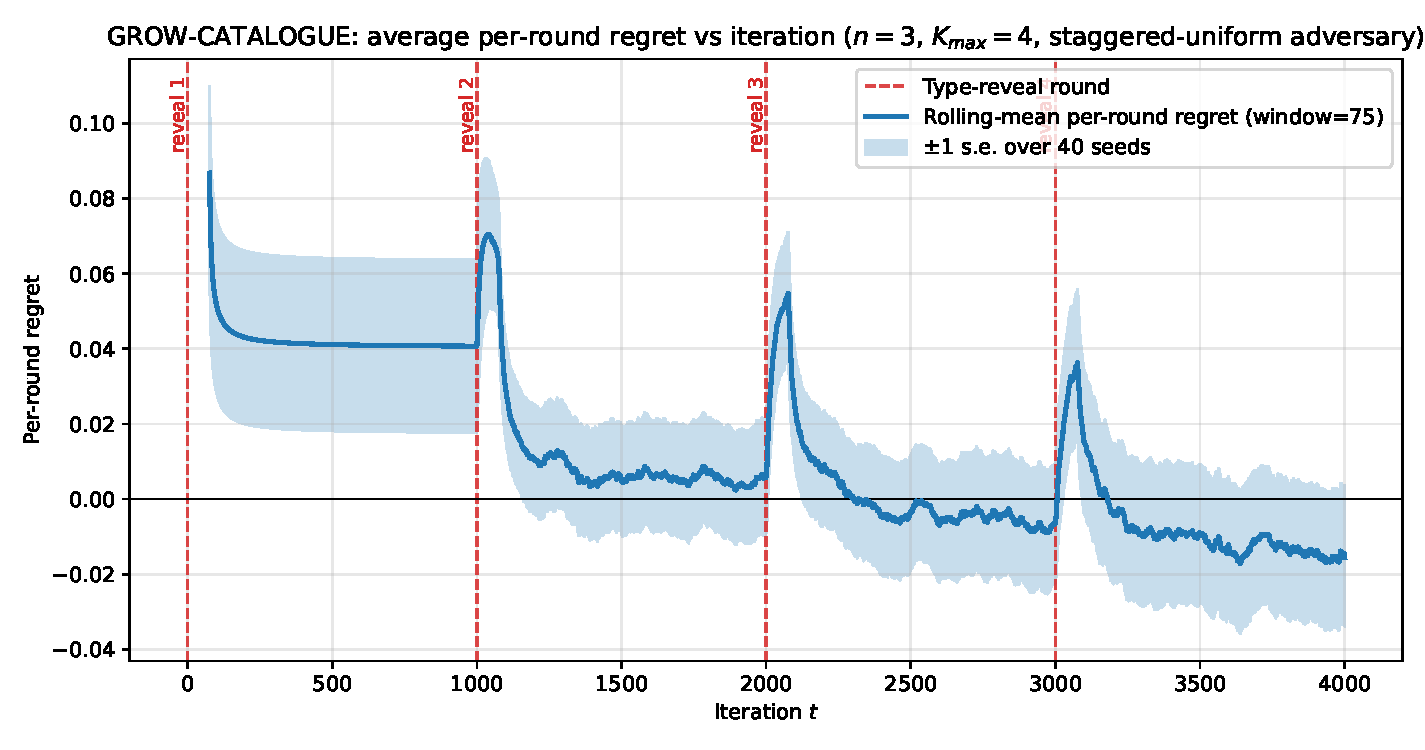
\includegraphics[width=0.98\linewidth]{figures/avg_regret_per_iter.pdf}
\vspace{-0.5em}
\caption{Rolling-window per-round regret of \textsc{Grow-Catalogue} under
the staggered-uniform adversary ($n=3$, $\Kmax=4$, $T=4000$, average over
$40$ seeds, window $=75$). Red dashed lines mark the discovery rounds
$0,1000,2000,3000$. Each reveal causes a visible transient spike,
followed by PW re-convergence inside the new epoch.}
\label{fig:per-round}
\end{figure}

\begin{figure}[t]
\centering
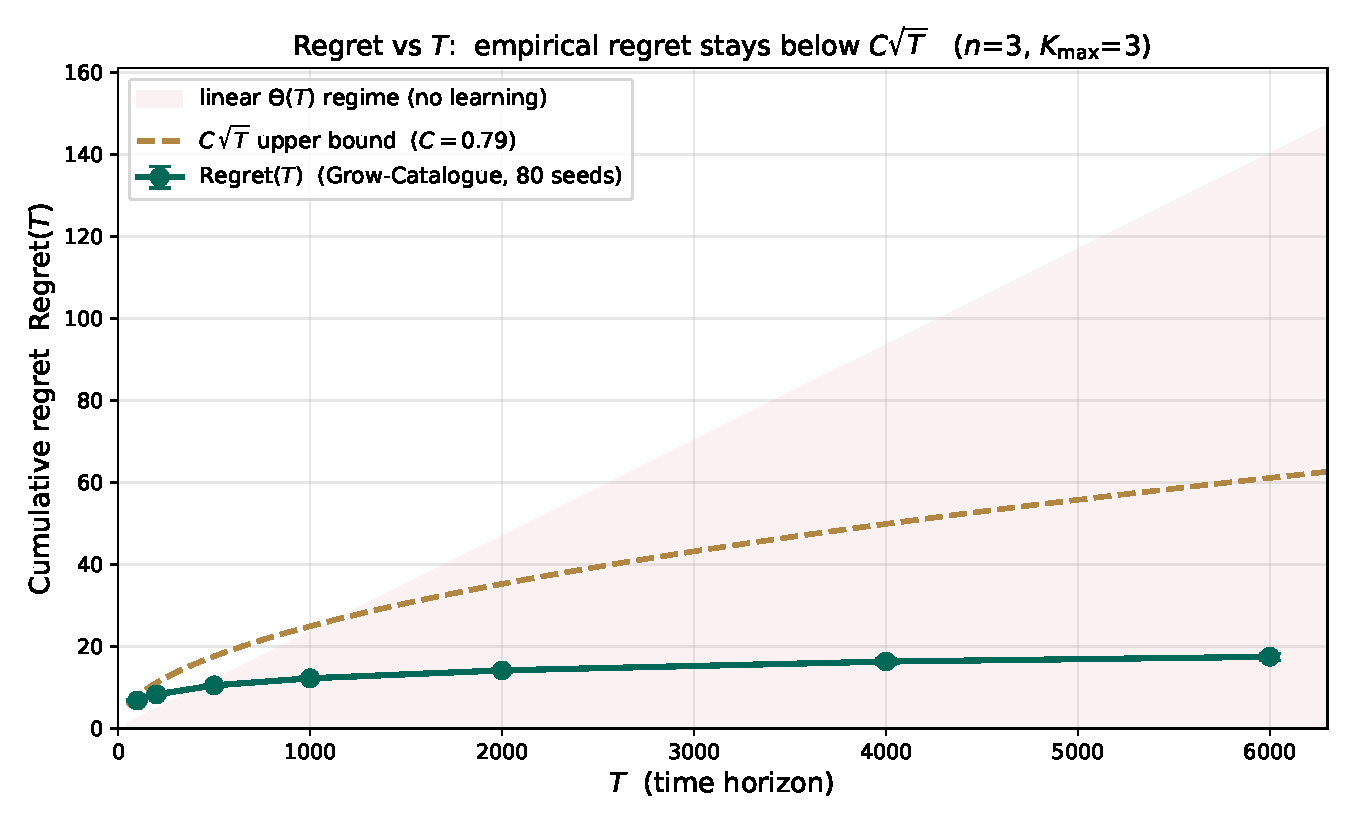
\includegraphics[width=0.98\linewidth]{figures/regret_vs_T_scaling.pdf}
\vspace{-0.5em}
\caption{Cumulative regret versus horizon $T$ for \textsc{Grow-Catalogue}
($n=3$, $\Kmax=3$, uniform random adversary, 80 seeds). The green curve
stays strictly below the $C\sqrt T$ upper envelope implied by
\Cref{thm:main}, which is in turn well below the linear-regret regime
that would result without learning.}
\label{fig:scaling}
\end{figure}

\Cref{fig:per-round} shows that the algorithm's per-round regret tracks
the epoch structure of the proof: each discovery round produces a bounded
transient, and the PW sub-routine re-converges within the new epoch. The
spikes shrink with $i$ because, by epoch $i$, the algorithm already has a
good PW distribution on most of the new (refined) extreme points.

\Cref{fig:scaling} plots cumulative $\Regret(T)$ versus $T$ with the
$C\sqrt T$ envelope from \Cref{thm:main} overlaid. The empirical regret
stays visibly below the envelope for all $T$ tested, and the ratio
$\Regret(T)/\sqrt T$ remains bounded (in fact, it decreases, indicating
that the stochastic staggered-uniform adversary is far from the worst
case). This is entirely consistent with \Cref{thm:main}, which is our upper bound

\Cref{tab:comparison} compares the four algorithms at $T=4000$. The regret
of \textsc{Grow-Catalogue} is
within roughly $15\%$--$40\%$ of the known-$K$ oracle and an order of
magnitude better than the uniform baseline. The two \textsc{Grow-Catalogue}
variants produce regret that differs only by Monte-Carlo noise, as
predicted by the observational equivalence of the two recomputation
schemes.

\begin{table}[h]
\centering
\footnotesize
\renewcommand{\arraystretch}{1.15}
\begin{tabular}{lcc}
\toprule
Algorithm & $\EE[\Regret(T)]$ & Ratio\\
\midrule
Known-$K$ oracle of \citet{balcan2015} & $14.51\pm 5.00$  & $1.00$\\
\textsc{Grow-Cat.} (total)     & $16.57\pm 5.40$  & $1.14$\\
Uniform baseline               & $292.77\pm 350.28$ & $20.18$\\
\bottomrule
\end{tabular}
\caption{Cumulative regret at $T=4000$, $n=3$, $\Kmax=3$, uniform-random
adversary, mean $\pm$ std over 15 seeds. The known-$K$ oracle receives
$K$ in advance; \textsc{Grow-Catalogue} attains comparable regret
\emph{without} this information.}
\label{tab:comparison}
\end{table}

% ==========================================================================
\section{Conclusions}
\label{sec:conc}

We studied the repeated Stackelberg security game in a new, open regime
in which the set of attacker types is unknown to the defender a priori
but known to have bounded cardinality. We presented \textsc{Grow-Catalogue},
a simple online algorithm that incrementally discovers attacker types and
re-partitions the coverage polytope accordingly, and we gave a full proof
that its expected regret under full-information feedback is at most
$O\!\bigl(\sqrt{T\cdot\Kmax\cdot(n^2+\Kmax\log n)}\bigr)$. This is the
same functional form as the known-$K$ bound of \citet[Theorem 5.1]{balcan2015},
with the known cardinality $k$ replaced by our known upper bound $\Kmax$.
The bound is sublinear whenever $\Kmax\cdot(n^2+\Kmax\log n)=o(T)$, and
the matching $\Omega(T)$ lower bound of \citet[Theorem 7.1]{balcan2015}
rules out further improvements on the unbounded side. Our experiments
confirm the analytical scaling: the empirical regret stays below the
$C\sqrt T$ envelope and tracks the epoch structure of the proof.



% ==========================================================================
% ===================  EXTENSION: SECTIONS 9-12  ===========================
% ==========================================================================

% Additional notation used only in the sections below.
\newcommand{\Univ}{\mathfrak{U}}
\newcommand{\cB}{\mathcal{B}}
\newcommand{\Ep}{\mathrm{Ep}}

\section{Partial-Information Feedback with an Unknown Type Set}
\label{sec:partial}

\Cref{prob:unknownK} pairs an \emph{unknown} attacker set $K$ with
\emph{full-information} feedback, and \Cref{thm:main} shows that the pairing
is benign: the price of not knowing $K$ is a factor $\sqrt{\Kmax}$ over the
known-$K$ rate of \citet[Theorem 5.1]{balcan2015}. \Citet[Section
6]{balcan2015} show that the other relaxation is benign as well: with $K$
\emph{known} but only the attacked target observed, regret
$O(T^{2/3}nk\log^{1/3}(nk))$ is achievable (their Theorem 6.1). It is natural
to expect that the two relaxations compose, and that the unknown-$K$ problem
under partial-information feedback admits a $T^{2/3}$-type bound with $k$
replaced by $\Kmax$.

This section shows that it does not, and that the failure is total: no
algorithm achieves regret $o(T)$, \emph{even when $\Kmax=1$}, i.e.\ even when
a single fixed attacker type attacks in every one of the $T$ rounds. The
obstruction is not the cardinality of $K$ --- it is that the defender can
never learn \emph{which} type it is facing, because the only thing it ever
observes is a target index, and the space of types that could have produced
that index is infinite.

\Cref{sec:partial,sec:block,sec:exp2,sec:conc2} extend the report in four
steps, and it is worth stating them together before starting.
\Cref{thm:impossible} is the impossibility just described.
\Cref{thm:bits} sharpens it into an exact accounting: on a universe of
$M$ candidate types, and given any oracle that emits at most $b$ bits over
the whole horizon, the optimal regret is $\min\{T,\log_2 M-b\}\pm 3$, so the
attainable regret is the number of bits still needed to name the attacker,
and no \emph{finite} budget helps on an infinite universe.
\Cref{prop:sqrtT} closes \Cref{sec:partial} by showing that this naming
account is exactly a $\Kmax=1$ phenomenon: two attacker types already force
$\Omega(\sqrt{T})$ on a two-element universe, under full information and with
$K$ known.
\Cref{sec:block} then fixes the model rather than the algorithm: an oracle
that every $B$ rounds reports the \emph{set} of types met so far restores
sublinear regret, at the rate
$\tilde O(n\Kmax^{4/3}T^{2/3}+\Kmax B)$ (\Cref{thm:block}), with the additive
term tight (\Cref{thm:blocklb}) and with a sharp separation between
scheduled and defender-chosen reporting times (\Cref{prop:adaptive}).
\Cref{sec:exp2} makes both algorithms oracle-efficient, which moves the
experiments from $n=3$ targets to $n=20$.

\subsection{The problem}
\label{sec:partial-problem}

\begin{problem}[Unknown-$K$ repeated SSG, partial information]
\label{prob:partial}
A repeated SSG as in \Cref{sec:model} is played, with three modifications.
\begin{enumerate}[leftmargin=1.2em,itemsep=0.05em,topsep=0.2em]
  \item There is a set $\Univ$ of attacker types, the \emph{universe}, which
  is known to the defender. It is not assumed to be finite;
  \Cref{thm:impossible} takes it infinite, while \Cref{thm:bits,prop:sqrtT}
  measure what happens when it is not.
  \item The set $K\subseteq\Univ$ of attacker types is not revealed to the
  defender at the start; however, the defender is given a constant
  $\Kmax\ge 1$ with the promise $|K|\le\Kmax$.
  \item Feedback is \emph{partial information} in the sense of
  \citet[Section 3]{balcan2015}: at the end of round $t$ the defender observes
  only the attacked target $b_{a_t}(\pvec_t)$. It never observes $a_t$, and
  the utility vectors of a type are never revealed.
\end{enumerate}
The adversary is oblivious, and the benchmark $\pvec^{*}$ and the regret
$\Regret(T)$ are as in \Cref{eq:pstar,eq:regret}.
\end{problem}

Two remarks fix the exact informational content of \Cref{prob:partial}.
First, the defender's own payoff is \emph{not} additional feedback: the
defender knows $u_d^c$ and $u_d^u$, so from the observed target
$i_t=b_{a_t}(\pvec_t)$ and its own $\pvec_t$ it computes
$U_d(i_t,\pvec_t)$ exactly. Second, \Cref{prob:partial} is at least as hard as
each of the two settings it weakens: \Cref{prob:unknownK} is recovered by
revealing $a_t$ and the utilities of each type on first contact, and the
setting of \citet[Section 6]{balcan2015} is recovered by revealing $K$ at
$t=0$.

\subsection{A three-target gadget}
\label{sec:gadget}

All lower bounds in this and the next section are proved in one fixed game,
which we call $G_3$ and which is the game of
\citet[Theorem 7.1]{balcan2015}, up to letting the single resource stand
idle. It has $n=3$ targets and one resource, with
schedules $\mathcal{D}=\{\emptyset,\{1\},\{2\},\{3\}\}$: the resource covers
one target or is left idle. The four pure strategies give
$\cP=\mathrm{conv}\{\mathbf{0},e_1,e_2,e_3\}
=\{\pvec\in[0,1]^3:p_1+p_2+p_3\le 1\}$. Allowing the resource to idle only
enlarges the defender's action set and therefore only strengthens the lower
bounds; every argument below also goes through verbatim on the simplex
$\{\pvec\ge 0:\sum_i p_i=1\}$ that one gets by forcing the resource to be
assigned, since each of the coverage vectors we exhibit has $\sum_i p_i=1$. The defender's payoffs are
\begin{equation}
u_d^c(i)=u_d^u(i)=-1\ \ (i\in\{1,3\}),\qquad u_d^c(2)=u_d^u(2)=0,
\label{eq:g3-def}
\end{equation}
so that by \Cref{eq:Ud}
\begin{equation}
U_d(1,\pvec)=U_d(3,\pvec)=-1,\qquad U_d(2,\pvec)=0
\label{eq:g3-payoff}
\end{equation}
for every $\pvec\in\cP$. Throughout \Cref{sec:partial,sec:block} the types
of $G_3$ break ties in favour of the lowest-indexed target, as in
\citet[Section 7]{balcan2015}; \Cref{sec:model} permits any fixed consistent
rule, and fixing one is part of specifying the instance. The choice is used
only to describe the feedback: at every coverage vector we exhibit as a
benchmark, the attacked target is the \emph{strict} maximizer, so the value
of the benchmark does not depend on the rule.

In $G_3$ the defender's payoff depends on
$\pvec_t$ \emph{only} through which target the attacker chooses: the round is
worth $0$ if target~$2$ is attacked and $-1$ otherwise. We say the defender
\emph{hits} at round $t$ if $b_{a_t}(\pvec_t)=2$ and \emph{misses} otherwise.

We now record the family of attacker types that $G_3$ admits. The statement
is \citet[Lemma 7.2]{balcan2015}; we give the utility vectors explicitly,
because the lower bounds below need the best response at \emph{every}
$\pvec\in\cP$ and not only on the segment considered there.

\begin{lemma}[realizable threshold types; cf.\ {\citealp[Lemma 7.2]{balcan2015}}]
\label{lem:realize}
For every pair $0\le r_1\le r_2\le 1$, the attacker type
$\alpha_{r_1,r_2}$ with utility vectors
\begin{equation}
u^c_{\alpha}=(r_1-1,\;0,\;-r_2),\qquad
u^u_{\alpha}=(r_1,\;0,\;1-r_2)
\label{eq:type-utils}
\end{equation}
has all its utilities in $[-1,1]$ and satisfies, for every $\pvec\in\cP$,
\begin{equation}
U_\alpha(1,\pvec)=r_1-p_1,\quad U_\alpha(2,\pvec)=0,\quad
U_\alpha(3,\pvec)=(1-r_2)-p_3 .
\label{eq:type-U}
\end{equation}
Consequently, if ties are broken in favour of the lowest-indexed target, the
restriction of $b_\alpha$ to the segment
$\{(p,0,1-p):p\in[0,1]\}$ is
\begin{equation}
b_{\alpha_{r_1,r_2}}\bigl((p,0,1-p)\bigr)=
\begin{cases}
1 & p\in[0,r_1],\\
2 & p\in(r_1,r_2],\\
3 & p\in(r_2,1].
\end{cases}
\label{eq:type-line}
\end{equation}
\end{lemma}

\begin{proof}
Since $0\le r_1\le r_2\le 1$ we have $r_1-1\in[-1,0]$, $-r_2\in[-1,0]$,
$r_1\in[0,1]$ and $1-r_2\in[0,1]$, so all six numbers in
\Cref{eq:type-utils} lie in $[-1,1]$ and $\alpha_{r_1,r_2}$ is a legitimate
attacker type in the sense of \Cref{sec:model}. For \Cref{eq:type-U},
substitute \Cref{eq:type-utils} into
$U_\alpha(i,\pvec)=u^c_\alpha(i)p_i+u^u_\alpha(i)(1-p_i)$:
\begin{align*}
U_\alpha(1,\pvec)&=(r_1-1)p_1+r_1(1-p_1)=r_1-p_1,\\
U_\alpha(2,\pvec)&=0\cdot p_2+0\cdot(1-p_2)=0,\\
U_\alpha(3,\pvec)&=-r_2p_3+(1-r_2)(1-p_3)=(1-r_2)-p_3 .
\end{align*}
On the segment $\pvec=(p,0,1-p)$ these read
$U_\alpha(1,\pvec)=r_1-p$, $U_\alpha(2,\pvec)=0$ and
$U_\alpha(3,\pvec)=p-r_2$. If $p\le r_1$ then $U_\alpha(1,\pvec)\ge 0$ and
$U_\alpha(3,\pvec)=p-r_2\le r_1-r_2\le 0$, so target~$1$ attains the maximum
(and wins any tie, being lowest-indexed). If $r_1<p\le r_2$ then
$U_\alpha(1,\pvec)<0$ and $U_\alpha(3,\pvec)\le 0=U_\alpha(2,\pvec)$, so
target~$2$ attains the maximum and wins the tie against target~$3$. If
$p>r_2$ then $U_\alpha(3,\pvec)>0=U_\alpha(2,\pvec)>U_\alpha(1,\pvec)$, and
target~$3$ is the strict maximizer.
\end{proof}

The next lemma is the structural fact that drives both lower bounds. It says
that in $G_3$ a hit is a very informative but very rare event: a coverage
vector hits at most one member of any family of types with disjoint
threshold intervals.

\begin{lemma}[the hit condition]
\label{lem:hit}
Let $0\le r_1<r_2\le 1$ and write $\alpha=\alpha_{r_1,r_2}$. For every
$\pvec\in\cP$,
\begin{equation}
b_\alpha(\pvec)=2
\iff
p_1>r_1\ \text{ and }\ p_3\ge 1-r_2 ,
\label{eq:hit-iff}
\end{equation}
and in that case $p_1\in(r_1,r_2]$. Consequently, if
$\{\alpha_{r_1^{(j)},r_2^{(j)}}\}_{j\in J}$ is any family of types whose
intervals $(r_1^{(j)},r_2^{(j)}]$ are pairwise disjoint, then for every
$\pvec\in\cP$ there is \emph{at most one} $j\in J$ with
$b_{\alpha_{r_1^{(j)},r_2^{(j)}}}(\pvec)=2$.
\end{lemma}

\begin{proof}
By \Cref{eq:type-U} and lowest-index tie-breaking, target~$2$ is chosen
exactly when $U_\alpha(2,\pvec)=0$ strictly beats $U_\alpha(1,\pvec)$ and
weakly beats $U_\alpha(3,\pvec)$, that is, when
$r_1-p_1<0$ and $(1-r_2)-p_3\le 0$; this is \Cref{eq:hit-iff}. If it holds,
then $p_1\le 1-p_2-p_3\le 1-p_3\le r_2$ because $\pvec\in\cP$ and
$p_2\ge 0$, so $p_1\in(r_1,r_2]$. The last claim follows because a single
$p_1$ cannot lie in two disjoint intervals.
\end{proof}

\subsection{Identification is a comparison search}
\label{sec:comparison}

Fix an integer $M\ge 2$ and let
\begin{equation}
I_j=\Bigl(\tfrac{j-1}{M},\tfrac{j}{M}\Bigr],\qquad
\alpha^{(j)}=\alpha_{\frac{j-1}{M},\frac{j}{M}},\qquad j\in[M],
\label{eq:dyadic}
\end{equation}
so that $I_1,\dots,I_M$ partition $(0,1]$ and
$\Univ_M\coloneqq\{\alpha^{(1)},\dots,\alpha^{(M)}\}$ is a set of $M$
distinct attacker types. \Cref{lem:hit} applies to $\Univ_M$ because the
$I_j$ are pairwise disjoint.

The defender's whole interaction with an instance $K=\{\alpha^{(j)}\}$ is
then a search for the index $j$ in which every query returns one of three
answers and the answer ``$2$'' is consistent with at most one candidate. The
following lemma bounds how fast \emph{any} such search can succeed. It
refines the classical $\Omega(\log_2 M)$ bound for comparison-based search in
three ways that the statements below need: it charges \emph{every}
unsuccessful query rather than only counting queries until termination; it
bounds the whole tail of the success time rather than its worst case; and it
allows the searcher to be fed, alongside the answers, an arbitrary side
channel of bounded total width. It is the combinatorial core of
\Cref{thm:impossible,thm:bits,thm:blocklb}, and is stated abstractly so that
it can be used three times.

\begin{lemma}[comparison trees identify slowly]
\label{lem:count}
Let $M\ge 1$, let $j$ be drawn uniformly at random from $[M]$, and fix a
\emph{side-information budget} $b\ge 0$. Consider any interactive protocol in
which, for $t=1,2,\dots$, a \emph{deterministic} strategy picks a query $q_t$
as a function of everything it has seen so far and then receives, in this
order, an answer $o_t=\mathcal{O}(q_t,j)\in\{1,2,3\}$ and a \emph{side
message} $\mu_t\in\Sigma_t$. The alphabets $\Sigma_0,\Sigma_1,\Sigma_2,\dots$
are fixed before play, $\mu_0\in\Sigma_0$ is delivered before the first query,
each $\mu_t$ may be an arbitrary function of $j$ and of the history, and the
total width of the side channel is bounded:
\begin{equation}
\sum_{t\ge 0}\log_2|\Sigma_t|\;\le\;b .
\label{eq:budget}
\end{equation}
Assume the single requirement that
\begin{equation}
\bigl|\{j'\in[M]:\mathcal{O}(q,j')=2\}\bigr|\le 1
\qquad\text{for every query } q .
\label{eq:one-hit}
\end{equation}
Let $\tau=\min\{t:o_t=2\}$, with $\tau=\infty$ if no such $t$ exists. Then
\begin{equation}
\Pr[\tau\le u]\;\le\;\frac{2^{b}\,(2^{u}-1)}{M}\qquad\text{for every } u\ge 1,
\label{eq:tau-tail}
\end{equation}
and consequently, for every $T\ge 1$,
\begin{equation}
\EE\bigl[\min\{\tau-1,\,T\}\bigr]\;\ge\;T-2^{b}\,\frac{2^{T+1}-T-2}{M}
\label{eq:count-final}
\end{equation}
and, in the cruder form that is easiest to read off,
\begin{equation}
\EE\bigl[\min\{\tau-1,\,T\}\bigr]\;\ge\;
\min\bigl\{T,\ \lfloor\log_2 M\rfloor-b\bigr\}-2 .
\label{eq:count-clean}
\end{equation}
Taking $b=0$, i.e.\ $|\Sigma_t|=1$ for every $t$, gives the side-channel-free
statement used in \Cref{thm:impossible,thm:blocklb}.
\end{lemma}

\begin{proof}
Fix $t\ge 1$ and let $H_t$ be the set of \emph{transcripts}
$(\mu_0,o_1,\mu_1,\dots,o_{t-1},\mu_{t-1})$ of the first $t-1$ rounds that
contain no answer $2$. Each such transcript has $o_s\in\{1,3\}$ for
$s\le t-1$ and $\mu_s\in\Sigma_s$ for $s\le t-1$, so by \Cref{eq:budget}
\[
|H_t|\;\le\;2^{t-1}\prod_{s=0}^{t-1}|\Sigma_s|\;\le\;2^{t-1}\,2^{b}.
\]
Suppose $\tau(j)=t$. Then the first $t-1$ rounds produced by $j$ form some
transcript $h\in H_t$, and, since the strategy is deterministic, the query
issued at round $t$ is the fixed query $q_t(h)$ determined by $h$; moreover
$\mathcal{O}(q_t(h),j)=2$. By \Cref{eq:one-hit} at most one index answers $2$
to $q_t(h)$, so for each $h\in H_t$ there is at most one $j$ with $\tau(j)=t$
and transcript $h$. As distinct $j$ with $\tau(j)=t$ must be counted under
some $h\in H_t$,
\[
\bigl|\{j\in[M]:\tau(j)=t\}\bigr|\;\le\;|H_t|\;\le\;2^{b}\,2^{t-1},
\]
and summing over $t\le u$ gives
$|\{j:\tau(j)\le u\}|\le 2^{b}\sum_{t=1}^{u}2^{t-1}=2^{b}(2^u-1)$. Dividing by
$M$ proves \Cref{eq:tau-tail}.

For \Cref{eq:count-final}, put $X=\min\{\tau-1,T\}$, a random variable with
values in $\{0,1,\dots,T\}$. For $0\le s\le T-1$ we have $X>s$ if and only if
$\tau-1>s$, i.e.\ $\tau>s+1$. Hence
\begin{align*}
\EE[X]&=\sum_{s=0}^{T-1}\Pr[X>s]
      =\sum_{u=1}^{T}\Pr[\tau>u]
      =\sum_{u=1}^{T}\bigl(1-\Pr[\tau\le u]\bigr)\\
      &\ge T-2^{b}\sum_{u=1}^{T}\frac{2^{u}-1}{M}
       = T-2^{b}\,\frac{2^{T+1}-2-T}{M},
\end{align*}
using $\sum_{u=1}^{T}2^u=2^{T+1}-2$.

For \Cref{eq:count-clean}, write $L=\lfloor\log_2 M\rfloor-b$. If $L\le 0$ the
claim is vacuous because $X\ge 0$. If $0<L$ and $T\le L$, then
$M\ge 2^{\lfloor\log_2 M\rfloor}=2^{L+b}$, so the subtracted term in
\Cref{eq:count-final} is at most
$2^{b}\,2^{T+1}/2^{L+b}=2^{\,T+1-L}\le 2$, giving $\EE[X]\ge T-2$. If
$0<L<T$, let $h=\lfloor L\rfloor$ and $f=L-h\in[0,1)$. Then $h\le T$ is an
integer and $X\ge\min\{\tau-1,h\}$ pointwise, so \Cref{eq:count-final} with
horizon $h$, together with $M\ge 2^{L+b}$, gives
$\EE[X]\ge h-2^{b}2^{h+1}/M=h-2^{\,1-f}$. Now $2-f\ge 2^{\,1-f}$ for every
$f\in[0,1)$: the two sides agree at $f=0$, and on $[0,1)$ the left side falls
with slope $-1$ while the right side falls with slope
$-2^{\,1-f}\ln 2\le-\ln 2>-1$. Hence $\EE[X]\ge h+f-2=L-2$. In all cases
$\EE[X]\ge\min\{T,L\}-2$; when $b$ is an integer and $M$ a power of two we
have $f=0$ and the middle step is the plain $2^{\,T+1-L}\le 2$ of the
previous case.
\end{proof}

\subsection{The impossibility theorem}
\label{sec:impossibility}

\begin{theorem}[unknown $K$ with partial information is not learnable]
\label{thm:impossible}
Let $G_3$ be the game of \Cref{eq:g3-def} and let
$\Univ=\{\alpha_{r_1,r_2}:0\le r_1\le r_2\le 1\}$ be the (infinite) universe
of threshold types of \Cref{lem:realize}. Then for every horizon $T\ge 1$ and
every $\Kmax\ge 1$, every online algorithm for \Cref{prob:partial} ---
randomized or deterministic, and even one that knows $T$, $\Univ$, $\Kmax$
and the construction below --- suffers, on some instance with $|K|=1$,
\begin{equation}
\EE[\Regret(T)]\;\ge\;T-2+\frac{T+2}{2^{T}}\;>\;T-2 .
\label{eq:impossible}
\end{equation}
The game $G_3$ does not depend on $T$; only the adversary's choice of $K$
inside the fixed universe $\Univ$ does.
\end{theorem}

\begin{proof}
Set $M=2^{T}$ and let $\Univ_M=\{\alpha^{(1)},\dots,\alpha^{(M)}\}\subset\Univ$
be as in \Cref{eq:dyadic}. Following the route of
\citet[Theorem 7.1]{balcan2015}, we invoke Yao's minimax principle: we
exhibit a distribution over instances and lower bound the expected regret of
every \emph{deterministic} algorithm against it.

\paragraph{The distribution over instances.}
Draw $j$ uniformly from $[M]$ and set $K=\{\alpha^{(j)}\}$ and
$a_t=\alpha^{(j)}$ for every $t\in[T]$. This is a legal instance of
\Cref{prob:partial} for every $\Kmax\ge 1$, since $|K|=1$; the sequence
$\avec$ is fixed before play begins, so the adversary is oblivious.

\paragraph{Step 1 (the benchmark is $0$).}
Let $\pvec^{*}=\bigl(\tfrac{2j-1}{2M},0,1-\tfrac{2j-1}{2M}\bigr)$, whose
first coordinate is the midpoint of $I_j$ and which lies in $\cP$. With
$r_1=\tfrac{j-1}{M}$ and $r_2=\tfrac{j}{M}$ we have
$p^{*}_1=\tfrac{2j-1}{2M}>\tfrac{2j-2}{2M}=r_1$ and
$p^{*}_3=1-\tfrac{2j-1}{2M}>1-\tfrac{2j}{2M}=1-r_2$, both strictly, so
\Cref{eq:hit-iff} gives $b_{\alpha^{(j)}}(\pvec^{*})=2$ --- and does so
under \emph{any} tie-breaking rule, since target~$2$ is the strict maximizer
at $\pvec^{*}$. Hence, by \Cref{eq:g3-payoff},
$U_d(b_{a_t}(\pvec^{*}),\pvec^{*})=0$ for every $t$. Since
$U_d(i,\pvec)\le 0$ for every target $i$ and every $\pvec$ by
\Cref{eq:g3-payoff}, no coverage vector can do better, so this $\pvec^{*}$ is
indeed a maximizer in \Cref{eq:pstar}. Therefore
$\sum_{t=1}^{T}U_d(b_{a_t}(\pvec^{*}),\pvec^{*})=0$, and by \Cref{eq:regret}
\begin{align}
\Regret(T)&=-\EE\Bigl[\sum_{t=1}^{T}U_d(b_{a_t}(\pvec_t),\pvec_t)\Bigr]\notag\\
&=\EE\bigl[\#\{t\le T:\text{miss at }t\}\bigr],
\label{eq:regret-is-misses}
\end{align}
again by \Cref{eq:g3-payoff}. So regret counts missed rounds exactly.

\paragraph{Step 2 (the interaction is a comparison search).}
A deterministic algorithm for \Cref{prob:partial} is a family of maps
$\pvec_t=\pvec_t(o_1,\dots,o_{t-1})$, where $o_s=b_{a_s}(\pvec_s)\in\{1,2,3\}$
is the only feedback it receives; its own past plays are determined by the
same history and carry no extra information, and as noted after
\Cref{prob:partial} its realized payoffs are functions of $(o_s,\pvec_s)$.
Define the query $q_t=\pvec_t$ and the answer map
$\mathcal{O}(\pvec,j')=b_{\alpha^{(j')}}(\pvec)$. The intervals $I_1,\dots,I_M$
are pairwise disjoint, so \Cref{lem:hit} gives exactly the hypothesis
\Cref{eq:one-hit}: for every $\pvec\in\cP$ at most one $j'\in[M]$ satisfies
$\mathcal{O}(\pvec,j')=2$. Hence the interaction is a protocol of the type
covered by \Cref{lem:count}, with budget $b=0$ because
\Cref{prob:partial} gives the defender no channel other than $o_t$.

\paragraph{Step 3 (counting).}
Let $\tau$ be the first round at which the algorithm hits. Every round
$t<\tau$ is a miss, and there are at least $\min\{\tau-1,T\}$ such rounds in
$[T]$. Combining with \Cref{eq:regret-is-misses} and \Cref{eq:count-final}
with $b=0$ and $M=2^{T}$,
\begin{align*}
\EE_j\bigl[\Regret(T)\bigr]&\;\ge\;\EE_j\bigl[\min\{\tau-1,T\}\bigr]\\
&\;\ge\;T-\frac{2^{T+1}-T-2}{2^{T}}\;=\;T-2+\frac{T+2}{2^{T}} .
\end{align*}

\paragraph{Step 4 (Yao).}
Let $A$ be any randomized algorithm and let $A_\omega$ denote its
deterministic realization under internal randomness $\omega$. Then
\begin{align*}
\max_{K,\avec}\EE[\Regret(T;A)]
&\;\ge\;\EE_j\EE_\omega[\Regret(T;A_\omega,j)]\\
&\;=\;\EE_\omega\EE_j[\Regret(T;A_\omega,j)],
\end{align*}
and the inner expectation is at least $T-2+(T+2)2^{-T}$ for every $\omega$ by
Steps 1--3. This proves \Cref{eq:impossible}.
\end{proof}

\begin{remark}[the bound is exactly tight]
\label{rem:tight-lb}
The constant in \Cref{eq:impossible} cannot be improved. The defender that
maintains the set of indices consistent with the observations so far --- an
integer interval, by \Cref{eq:type-line} --- and plays
$\pvec_t=(k/M,0,1-k/M)$ for its midpoint $k$ attains expected regret exactly
$T-2+(T+2)2^{-T}$ on this family, as we verify in \Cref{sec:exp-imp}. Since
$\Regret(T)\le T$ always in $G_3$, \Cref{thm:impossible} says the defender
loses all but two of the $T$ rounds.
\end{remark}

\subsection{What exactly fails, and what would fix it}
\label{sec:whatfails}

\Cref{thm:impossible} is not a statement about how many types the adversary
has; the hard instance uses a single type, deployed in every round. It is a
statement about how many types the adversary \emph{could} have had. The next
theorem makes that precise by re-running the argument on a universe of finite
resolution, exhibiting a matching algorithm, and --- since the diagnosis is
that the defender is missing the \emph{name} of a type --- pricing the
supplement that would repair it. We charge that supplement in bits.

\begin{definition}[side-information oracle of budget $b$]
\label{def:budget}
A \emph{side-information oracle of budget $b$} for \Cref{prob:partial} is
given by alphabets $\Sigma_0,\Sigma_1,\dots,\Sigma_T$ fixed before play with
$\sum_{t}\log_2|\Sigma_t|\le b$, together with message maps that hand the
defender $\mu_0\in\Sigma_0$ before round~$1$ and $\mu_t\in\Sigma_t$ at the end
of round $t$. Each $\mu_t$ may be an arbitrary function of the instance
$(K,\avec)$ and of the history so far. Nothing is assumed about what the
messages mean; $b$ measures only how many bits of them there are.
\end{definition}

\begin{theorem}[regret is the number of bits needed to name the type]
\label{thm:bits}
Fix $M\ge 2$ and a budget $b\ge 0$, and consider \Cref{prob:partial} in
$G_3$ with $\Kmax=1$, augmented by a side-information oracle of budget $b$.
Parts (i) and (iii) hold for every real $b\ge 0$; part (ii), which has to
build $2^{b}$ blocks, is stated for integer $b$.
\begin{enumerate}[leftmargin=1.2em,itemsep=0.05em,topsep=0.2em]
  \item On the universe $\Univ_M$ of \Cref{eq:dyadic}, every algorithm and
  every such oracle suffer
  $\EE[\Regret(T)]\ge\min\{T,\lfloor\log_2 M\rfloor-b\}-2$
  on some instance.
  \item For integer $b$, on $\Univ_M$ there are an oracle of budget $b$ and an
  algorithm that
  together suffer
  $\Regret(T)\le\min\bigl\{T,\ \max\{0,\lceil\log_2 M\rceil-b\}\bigr\}$
  on every instance.
  \item On the infinite universe $\Univ$ of \Cref{thm:impossible}, every
  algorithm and every oracle of \emph{any} finite budget $b$ suffer
  $\EE[\Regret(T)]\ge T-2$ on some instance with $|K|=1$.
\end{enumerate}
Hence on $\Univ_M$ the optimal regret is $\min\{T,\log_2 M-b\}\pm 3$ --- and
$\pm 2$ when $M$ is a power of two, which is the only case used below --- so
one bit of threat intelligence buys exactly one round, until the type has
been named and the remaining rounds are free. Taking $b=0$ recovers the statement that
the optimal regret is $\min\{T,\log_2|\Univ_M|\}\pm 3$, and (iii) says that
on an infinite universe no fixed quantity of intelligence buys anything at
all.
\end{theorem}

\begin{proof}
(i) Repeat Steps~1--4 of the proof of \Cref{thm:impossible} on $\Univ_M$
verbatim; the only change is in Step~2, where the protocol handed to
\Cref{lem:count} now also carries the messages $\mu_t$, so it is a protocol
of budget $b$ rather than $0$. Note that \Cref{lem:count} allows $q_t$ to
depend on $\mu_0,\dots,\mu_{t-1}$, which is exactly the freedom a defender
reading the oracle has, and that \Cref{eq:one-hit} is a property of the
answer map $\mathcal{O}$ alone and is therefore untouched by the side
channel. Step~3 now invokes \Cref{eq:count-clean} instead of
\Cref{eq:count-final} and gives
$\EE_j[\Regret(T)]\ge\min\{T,\lfloor\log_2 M\rfloor-b\}-2$ for every
deterministic algorithm; Step~4 is unchanged.

(ii) Write $m=\lceil\log_2 M\rceil$. If $b\ge m$ let the oracle name $j$
outright, using $\lceil\log_2 M\rceil\le b$ bits, and let the defender play
the midpoint of $I_j$ forever; by \Cref{eq:hit-iff} it hits in every round
and the regret is $0$. Otherwise split $[M]$ into $2^{b}$ consecutive blocks
of $\lceil M/2^{b}\rceil$ or fewer indices each and let $\mu_0$ name the
block containing $j$; this is one message from an alphabet of size $2^{b}$,
so the budget is met. The defender then runs the midpoint search of
\Cref{rem:tight-lb} restricted to that block: it keeps the sub-interval
$[\ell,h]$ of indices consistent with everything it has seen, initially the
announced block, and plays $\pvec=(k/M,0,1-k/M)$ for its midpoint $k$. By
\Cref{eq:type-line} at that $\pvec$, the observation is target~$2$ if $j=k$,
target~$1$ if $j>k$ and target~$3$ if $j<k$, so every missed round replaces
$[\ell,h]$ by one of its two halves and every hit leaves it unchanged.
Starting from $\lceil M/2^{b}\rceil\le 2^{\,m-b}$ candidates, at most $m-b$
misses can occur before $[\ell,h]$ is a singleton, after which every round is
a hit; and trivially at most $T$ rounds are missed. By
\Cref{eq:regret-is-misses} the regret equals the number of misses.

(iii) Apply (i) on the sub-universe $\Univ_{M}\subset\Univ$ with
$M=2^{T+b}$, for which $\lfloor\log_2 M\rfloor-b=T$; the instance produced
has $|K|=1$.
\end{proof}

\begin{remark}[what the budget does and does not cover]
\label{rem:budget}
\Cref{def:budget} is deliberately permissive: the oracle may look at the
whole instance, may speak before the game starts, may adapt its messages to
the defender's plays, and is free to use any encoding at all. What it may
not do is exceed $b$ bits in total. The lower bound is therefore
information-theoretic and not an artefact of any particular reporting format;
in particular it applies to the block-revelation oracle of \Cref{sec:block}
whenever that oracle's messages can be encoded in $b$ bits. What
\Cref{thm:bits} does \emph{not} capture is \emph{when} the bits arrive:
\Cref{thm:blocklb} below shows that even an oracle with a generous budget
still costs $\Theta(\Kmax B)$ if it is made to speak only every $B$ rounds.
Volume and latency are two independent obstructions, and the two lower
bounds isolate them one at a time.
\end{remark}

\begin{remark}[the two lower bounds are incomparable]
\label{rem:contrast}
\Cref{tab:landscape} places \Cref{thm:impossible} among the known results.
\Citet[Theorem 7.1]{balcan2015} obtain $\Omega(T)$ with \emph{full}
information, but their construction uses a type set of size $2^{T+1}-2$, and
the sequence it plays --- the $T$ postfixes of a random $T$-bit string ---
contains $T$ \emph{distinct} types, so it needs $\Kmax\ge T$ and is
consistent with \Cref{thm:main}. \Cref{thm:impossible} obtains $\Omega(T)$
with $|K|=1$, and hence for every $\Kmax\ge 1$, but needs partial
information and an infinite universe. Neither implies the other. Together
with \Cref{thm:main} and \citet[Theorem 6.1]{balcan2015} they show that
either relaxation of \citet[Theorem 5.1]{balcan2015} alone is affordable ---
a $\sqrt{\Kmax}$ multiplicative price for not knowing $K$, an exponent
$2/3$ instead of $1/2$ for not observing $a_t$ --- while their conjunction is
not affordable at all.
\end{remark}

\begin{table}[t]
\centering
\footnotesize
\renewcommand{\arraystretch}{1.2}
\begin{tabular}{@{}lll@{}}
\toprule
Feedback & Set $K$ & Regret\\
\midrule
full    & known, $|K|=k$        & $O(\sqrt{Tn^2k\log nk})$\\
partial & known, $|K|=k$        & $O(T^{2/3}nk\log^{1/3}\!nk)$\\
full    & known, $|K|=2^{T+1}{-}2$ & $\Omega(T)$\\
full    & unknown, $\le\Kmax$   & $O(\sqrt{T\Kmax\Lambda_n})$\\
partial & unknown, $\le\Kmax$   & $\Omega(T)$, even $\Kmax{=}1$\\
partial & unknown, $\Kmax{=}1$, & \\
        & \ \ $|\Univ|{=}M$, $b$ bits & $\min\{T,\log_2 M-b\}\pm 3$\\
full    & known, $|K|{=}|\Univ|{=}2$ & $\Theta(\sqrt T)$\\
partial & unknown, $\le\Kmax$,  & \\
        & \ \ block revelation  & $\tilde O(n\Kmax^{4/3}T^{2/3}{+}\Kmax B)$\\
\bottomrule
\end{tabular}
\caption{The landscape, with $\Lambda_n=n^2+\Kmax\log n$. Rows 1--3 are
Theorems 5.1, 6.1 and 7.1 of \citet{balcan2015}; row 4 is \Cref{thm:main};
row 5 is \Cref{thm:impossible}; row 6 is \Cref{thm:bits}, which is tight up
to an additive $3$; row 7 is \Cref{prop:sqrtT} together with \Cref{thm:main}
at $k=2$, and is tight up to a constant. The $\Omega(\sqrt T)$ half of row 7
holds under partial information as well, but the matching upper bound does
not: with partial information the best bound we can cite for a known
two-type set is the $O(T^{2/3})$ of \citet[Theorem 6.1]{balcan2015}, and
closing that gap is one of the open problems of \Cref{sec:conc2}. Row 8 is
\Cref{thm:block}, in the model of \Cref{prob:block}.}
\label{tab:landscape}
\end{table}

\begin{remark}[the adversary is not the difficulty]
\label{rem:stationary}
The instance of \Cref{thm:impossible} is stationary: one fixed type attacks
in every round. The lower bound therefore continues to hold if the defender
is additionally told $|K|$ exactly, told the full frequency vector of the
type sequence, or told that the sequence is i.i.d.; none of these is
informative when $|K|=1$. What the defender is missing is not information
about \emph{which types attack when}, which is the quantity that
\citet[Section 6]{balcan2015} must estimate, but information about the
identity of the types themselves.
\end{remark}

\begin{remark}[reconciliation with query-based learning]
\label{rem:letchford}
\Citet{letchford2009} show that a defender facing a \emph{single} unknown
attacker type can learn a near-optimal commitment from a small number of
best-response queries, which at first sight is in tension with
\Cref{thm:impossible}. There is no contradiction. Any query bound of that
kind must depend on the geometry of the best-response regions, and the family
$\Univ_M$ of \Cref{eq:dyadic} drives the region that has to be located down
to width $1/M=2^{-T}$. \Cref{thm:bits} says exactly that a dependence
of this kind cannot be removed: the attainable regret is the number of bits
needed to name the attacker type, and an infinite universe makes that number
unbounded.
\end{remark}

\subsection{A $\sqrt{T}$ floor as soon as $\Kmax\ge 2$}
\label{sec:floor}

\Cref{thm:bits} makes the $\Kmax=1$ problem entirely a naming problem: on a
universe of resolution $M$ the regret is $\min\{T,\log_2 M-b\}\pm 3$, which
for a fixed finite universe does not grow with the horizon at all. The next
proposition shows that this is a property of $\Kmax=1$ and of nothing else.
With two attacker types the regret is $\Omega(\sqrt{T})$ on the
\emph{smallest possible} universe, under \emph{full}-information feedback,
and even if the defender is told $K$ in advance. Two consequences are worth
naming. First, the $\sqrt{T}$ of \Cref{thm:main} is not an artefact of the
analysis. Second, whatever the answer to the finite-$M$ question of
\Cref{sec:conc2} turns out to be for $\Kmax\ge 2$, it must keep growing with
the horizon, and so it cannot have the saturating form
$\min\{T,f(M,\Kmax)\}$ that governs $\Kmax=1$.

\begin{proposition}[two types already cost $\sqrt{T}$]
\label{prop:sqrtT}
Consider $G_3$ with the two attacker types
$\alpha^{(1)}=\alpha_{0,1/2}$ and $\alpha^{(2)}=\alpha_{1/2,1}$ of
\Cref{lem:realize}, so that $|\Univ|=|K|=\Kmax=2$. Let $a_1,\dots,a_T$ be
drawn i.i.d.\ and uniformly from $K$. Then every online algorithm ---
randomized or deterministic, under full information or partial information,
and even one that is told $K$ together with the utility vectors at $t=0$ ---
satisfies
\begin{equation}
\EE\bigl[\Regret(T)\bigr]\;\ge\;\tfrac{1}{2}\sqrt{\lfloor T/2\rfloor}
\label{eq:sqrtT}
\end{equation}
for every $T\ge 2$, where the expectation is over the sequence as well as the
algorithm's randomization; consequently some fixed sequence forces at least
this much.
\end{proposition}

\begin{proof}
The intervals $(0,\tfrac12]$ and $(\tfrac12,1]$ of the two types are
disjoint, so \Cref{lem:hit} applies: every $\pvec\in\cP$ hits at most one of
$\alpha^{(1)},\alpha^{(2)}$. Write $N_i=|\{t:a_t=\alpha^{(i)}\}|$, so
$N_1+N_2=T$.

\emph{The benchmark.} A fixed $\pvec$ earns $0$ on the rounds at which it
hits and $-1$ on the others, by \Cref{eq:g3-payoff}, and by the previous
paragraph it hits on at most $\max\{N_1,N_2\}$ rounds. That value is
attained: $\pvec=(\tfrac14,0,\tfrac34)$ satisfies $p_1>0$ and
$p_3\ge\tfrac12$, so by \Cref{eq:hit-iff} it hits $\alpha^{(1)}$ in every one
of its $N_1$ rounds, and symmetrically $\pvec=(\tfrac34,0,\tfrac14)$ hits
$\alpha^{(2)}$ in every one of its $N_2$ rounds. Hence
$\sum_t U_d(b_{a_t}(\pvec^{*}),\pvec^{*})=-\min\{N_1,N_2\}$.

\emph{The algorithm.} Fix a round $t$ and condition on the algorithm's
history, which is a function of $a_1,\dots,a_{t-1}$ and of its internal
randomization and is therefore independent of $a_t$. The played $\pvec_t$
hits at most one of the two types, and $a_t$ equals that type with
probability $\tfrac12$; so $\Pr[\text{hit at }t]\le\tfrac12$ conditionally,
hence unconditionally. Summing,
$\EE[\sum_t U_d(b_{a_t}(\pvec_t),\pvec_t)]=-\,\EE[\#\text{misses}]\le -T/2$.

\emph{Combining.} Since $\min\{N_1,N_2\}=\tfrac12(T-|N_1-N_2|)$,
\[
\EE[\Regret(T)]\;\ge\;\tfrac{T}{2}-\EE\bigl[\min\{N_1,N_2\}\bigr]
\;=\;\tfrac{1}{2}\,\EE\bigl[\,|N_1-N_2|\,\bigr].
\]
Now $N_1-N_2=S_T\coloneqq\sum_{t\le T}\varepsilon_t$ with
$\varepsilon_t=\pm1$ independent and uniform. The process $|S_m|$ is a
submartingale, so $\EE|S_T|\ge\EE|S_{2\nu}|$ with $\nu=\lfloor T/2\rfloor$,
and the classical identity
$\EE|S_{2\nu}|=2\nu\binom{2\nu}{\nu}4^{-\nu}$ together with
$\binom{2\nu}{\nu}4^{-\nu}\ge 1/(2\sqrt{\nu})$ gives
$\EE|S_T|\ge\sqrt{\nu}$. (The inequality
$\binom{2\nu}{\nu}4^{-\nu}\ge1/(2\sqrt\nu)$ holds with equality at $\nu=1$
and follows by induction, since the ratio of consecutive left-hand sides is
$(2\nu+1)/(2\nu+2)$ and that of right-hand sides is $\sqrt{\nu/(\nu+1)}$,
and $(2\nu+1)^2(\nu+1)\ge \nu(2\nu+2)^2$ reduces to $\nu+1\ge0$.)
This is \Cref{eq:sqrtT}. Nothing in the argument refers to the feedback
model or to knowledge of $K$: the only facts used are that $\pvec_t$ cannot
hit both types and that $a_t$ is independent of the past.
\end{proof}

The bound is tight on this instance, and in a strong sense: the inequality
$\Pr[\text{hit at }t]\le\tfrac12$ is an equality for any algorithm that
always plays inside one of the two intervals, so every such algorithm ---
including follow the leader, and including one that is simply told $K$ ---
has expected regret \emph{exactly} $\tfrac12\EE|N_1-N_2|$, which is
$\sqrt{T/(2\pi)}\,(1+o(1))$. The remaining freedom buys nothing at all.
\Cref{fig:impossible}(c) shows the measured curve sitting on that value.

\begin{remark}[the phase transition at $\Kmax=2$]
\label{rem:phase}
\Cref{thm:bits,prop:sqrtT} bracket the finite-universe problem from two
sides. With $\Kmax=1$ the regret is $\min\{T,\log_2 M\}\pm 3$ and stops
growing once the type has been named. With $\Kmax=2$ it is
$\Omega(\sqrt{T})$ even at $M=2$, because the defender must now track which
of its two known opponents is currently more frequent, and no naming can
settle that. The transition is therefore not about how hard it is to
identify a type but about whether identification is the whole problem. On
the upper side, \citet[Theorem 6.1]{balcan2015} run with $k=M$ --- legitimate
here, since a finite universe \emph{is} a known type set --- gives
$O(\min\{T,\,T^{2/3}nM\log^{1/3}(nM)\})$ under partial information, and
\Cref{thm:main} gives $O(\sqrt{T\Kmax(n^2+\Kmax\log n)})$ under full
information. Closing the gap between $\Omega(\sqrt T)$ and these is the
finite-$M$ question of \Cref{sec:conc2}.
\end{remark}

% ==========================================================================
\section{Block Revelation: Recovering Sublinear Regret}
\label{sec:block}

\Cref{thm:impossible} says that the defender must be told \emph{something}
about the identity of its opponents. \Cref{thm:bits} says how little
may suffice: what the defender is missing is the name of a type, and a name
is a bounded object. This section studies the weakest such supplement we
could find that is realistic in the applications of \Cref{sec:intro} --- a
periodic threat-intelligence report --- and shows that it restores sublinear
regret at the partial-information rate of \citet[Theorem 6.1]{balcan2015}.

The supplement is deliberately meagre. Every $B$ rounds, an oracle hands the
defender the \emph{set} of attacker types that have attacked at least once so
far, together with their utility vectors. It does not say when any of them
attacked, how often, or how many are still to come. In particular the
defender still cannot attribute any individual round to a type, which is
precisely the difficulty that \citet[Section 6]{balcan2015} solve by
estimating type frequencies from best responses; that difficulty is
untouched, and it is why the rate below is $T^{2/3}$ rather than $\sqrt{T}$.

\subsection{The model}

\begin{problem}[Unknown-$K$ repeated SSG with block revelation]
\label{prob:block}
Fix a \emph{revelation length} $B\in\NN$, known to the defender, and
partition the horizon into $N_B=\lceil T/B\rceil$ \emph{revelation blocks}
\begin{equation}
\cB_\nu=\{(\nu-1)B+1,\ \dots,\ \min\{\nu B,T\}\},\qquad \nu\in[N_B].
\label{eq:blocks}
\end{equation}
The game is \Cref{prob:partial}, with one addition: at the end of block
$\cB_\nu$ the defender is given the set
\begin{equation}
D_\nu\;=\;\{a_t\ :\ t\le \min\{\nu B,T\}\}\ \subseteq\ K
\label{eq:Dnu}
\end{equation}
of types that have attacked so far, together with the utility vectors
$(u^c_\alpha,u^u_\alpha)$ of each $\alpha\in D_\nu$. We set $D_0=\emptyset$.
Nothing else is revealed: not $|K|$, not the rounds at which any type
attacked, and not the number of times any type attacked. Within a round the
feedback is still partial information.
\end{problem}

Three observations delimit \Cref{prob:block}. First, it is strictly weaker
than \Cref{prob:unknownK}: even at $B=1$ the defender learns the type of
round $t$ only when that type is new, and on every other round it still sees
nothing but a target. Second, $B\ge T$ makes the revelation useless and
recovers \Cref{prob:partial}, so by \Cref{thm:impossible} some bound on $B$
is necessary; \Cref{thm:blocklb} below quantifies this. Third, the oracle is
\emph{cumulative} rather than incremental --- it reports the whole set
$D_\nu$, not the increment $D_\nu\setminus D_{\nu-1}$ --- but the two are
equivalent for a defender that remembers $D_{\nu-1}$, and we use whichever is
more convenient.

\subsection{The algorithm}

\Cref{alg:bgc} is \Cref{alg:gc} with two changes forced by the model: the
catalogue is refreshed at checkpoints rather than at discovery rounds, and
the inner learner is the partial-information algorithm of
\citet[Algorithm 1]{balcan2015} rather than Polynomial Weights, because the
loss of an expert can no longer be computed from the feedback. We write
$\mathcal{A}(C)$ for a fresh instance of that algorithm run on the
$\epsilon$-approximate extreme-point set $\cE(C;\epsilon)$ with attacker set
$C$; as there, $\mathcal{A}(C)$ spends $|C|$ rounds of each of its internal
estimation blocks playing the barycentric-spanner strategies and the rest
playing the strategy proposed by its full-information sub-routine. We fix
$\epsilon=1/T$ once and for all rather than tuning it to a segment length.
This is admissible for every segment, because the discretization error of
\Cref{lem:43} is $2\epsilon L$ and so only decreases with $\epsilon$, while
the size bound of \Cref{lem:44} does not depend on $\epsilon$ at all; and it
is convenient, because it lets a single expert set serve a catalogue for the
whole horizon.

One property of $\mathcal{A}(C)$ that the proof of \Cref{thm:main} obtained
for free has to be arranged explicitly here. There the inner learner was
Polynomial Weights, which by \Cref{prop:hedge} is \emph{anytime}, so the fact
that an epoch's length is revealed only when the epoch ends cost nothing.
The algorithm of \citet[Theorem 6.1]{balcan2015}, by contrast, tunes its
number of estimation blocks to a horizon supplied in advance, and the epochs
of \Cref{def:blocks} again have lengths that the defender does not know when
they begin. The following lemma supplies the anytime form that
\Cref{thm:block} will use. Its proof takes \citet[Theorem 6.1]{balcan2015}
as a black box except for one structural feature of the proof of their
Lemma 6.2, which we quote rather than repeat.

\begin{lemma}[an anytime partial-information learner]
\label{lem:anytime}
Let $C$ be a finite catalogue, let $T$ be the horizon of \Cref{prob:block},
and let $\epsilon\le 1/T$. There is an algorithm $\mathcal{A}(C)$ for the
partial-information setting with known attacker set $C$, running over
$\cE(C;\epsilon)$ and not receiving its own horizon in advance, and an
absolute constant $c_2$ (distinct from the $c_1$ of \Cref{sec:proof}), such
that for every oblivious sequence
$a'_1,a'_2,\dots$ with $a'_t\in C$ for all $t$ and for \emph{every}
$1\le L\le T$ simultaneously,
\begin{align}
&\max_{\pvec\in\cP}\sum_{t=1}^{L}U_d\bigl(b_{a'_t}(\pvec),\pvec\bigr)
 -\EE\Bigl[\sum_{t=1}^{L}U_d\bigl(b_{a'_t}(\pvec_t),\pvec_t\bigr)\Bigr]\notag\\
&\hspace{5em}\le\;c_2\,L^{2/3}\,n\,|C|\,\log^{1/3}\!\bigl(n|C|\bigr).
\label{eq:anytime}
\end{align}
\end{lemma}

\begin{proof}
\emph{(a) The bound of \citet[Theorem 6.1]{balcan2015} already holds at every
prefix of a run tuned to a horizon $H$.} Their algorithm divides $[1,H]$ into
$Z=n\bigl(H^{2}\log(n|C|)\bigr)^{1/3}$ estimation blocks of $H/Z$ rounds
each, with $Z$ a function of $H$, $n$ and $|C|$ only. Dispose first of the
degenerate range $Z\ge H$, in which there are not enough rounds to form the
blocks at all: that range is $H\le n^{3}\log(n|C|)$, and there the trivial
bound of two per round gives regret at most $2H=2H^{1/3}\cdot H^{2/3}\le
2n\log^{1/3}(n|C|)\,H^{2/3}$, which is below the claim for any $c_0\ge 2$.
So assume $Z\le H$. The chain of inequalities in their proof of Lemma 6.2 bounds
the algorithm's loss over the first $\tau_0$ blocks by the loss of the best
fixed action over those same blocks plus
\[
\tfrac{H}{Z}\,R_{\tau_0,\kappa}\;+\;\tau_0\,|C| ,
\]
where $\kappa=n|C|$ is the range of the loss estimator
\citep[Lemma 6.4]{balcan2015}, $R_{\tau_0,\kappa}$ is the regret of the
full-information sub-routine after $\tau_0$ estimated loss vectors, and the
term $\tau_0|C|$ pays for the $|C|$ exploration rounds of each block. Both
summands are non-decreasing in $\tau_0$ and are maximized at $\tau_0=Z$; and
the sub-routine of \Cref{prop:hedge} is anytime, so
$R_{\tau_0,\kappa}=O(\sqrt{\tau_0\,\kappa\log|\cE(C;\epsilon)|})$ holds for
every $\tau_0$ and not only for $\tau_0=Z$. Reading the chain at an arbitrary
$\tau_0\le Z$ therefore reproduces their bound with $H$ in place of $T$. A
prefix that stops inside a block contributes at most two per round for the at
most $H/Z$ rounds of that block, and $H/Z\le H^{2/3}n|C|\log^{1/3}(n|C|)$, so
this is absorbed. The discretization error incurred by optimizing over
$\cE(C;\epsilon)$ instead of $\cP$ is $2\epsilon L\le 2$ by \Cref{lem:43} and
$\epsilon\le 1/T$, and is absorbed as well; note that $\epsilon$ enters the
size bound of \Cref{lem:44} not at all, so taking it smaller than
\citet{balcan2015} do is free. Hence there is an absolute constant $c_0$ such
that a run tuned to $H$ satisfies \Cref{eq:anytime} with $L^{2/3}$ replaced by
$H^{2/3}$, simultaneously for every $L\le H$.

\emph{(b) Doubling.} Write $\phi=n|C|\log^{1/3}(n|C|)$ for the
catalogue-dependent factor in \Cref{eq:anytime}, and let $\mathcal{A}(C)$ run
in stages $s=0,1,2,\dots$, where stage $s$ occupies $2^{s}$ consecutive rounds
and is a fresh instance tuned to the horizon $H_s=2^{s}$. Fix $L$ and let $S$
be the stage containing round $L$. Stages $0,\dots,S-1$ occupy $2^{S}-1$
rounds, all of them at most $L$, so $2^{S}\le L$. For any $\pvec\in\cP$ the
sum over $[1,L]$ splits across stages, so the maximum over $\cP$ of the sum is
at most the sum over stages of the per-stage maxima; subtracting the
algorithm's payoff stage by stage gives
\[
R_{[1,L]}\;\le\;\sum_{s=0}^{S}R^{(s)} ,
\]
where $R^{(s)}$ denotes the regret of the instance of stage $s$ over that
part of stage $s$ which lies in $[1,L]$. Each $R^{(s)}$ is bounded by (a)
with $H=2^{s}$ --- the restriction of an oblivious sequence to a stage is
oblivious and still takes values in $C$ --- so
\[
R_{[1,L]}\;\le\;c_0\,\phi\sum_{s=0}^{S}2^{2s/3}
\;\le\;\frac{2^{2/3}}{2^{2/3}-1}\;c_0\,\phi\;2^{2S/3},
\]
and $2^{S}\le L$ gives \Cref{eq:anytime} with
$c_2=2^{2/3}c_0/(2^{2/3}-1)<2.71\,c_0$.
\end{proof}

One caveat about the factor $n|C|$ in \Cref{eq:anytime} should be recorded,
since \Cref{lem:anytime} is the one place in this report where the proof of
\citet[Theorem 6.1]{balcan2015} is reopened rather than quoted. That factor
is inherited, through their Lemma 6.2, from the form
$R_{L',\kappa}\le\sqrt{L'\kappa\log|\cM|}$ in which \Cref{prop:hedge} states
the full-information guarantee for losses of range $\kappa$. The textbook
guarantee for Polynomial Weights on losses in $[-\kappa,\kappa]$ is instead
$O(\kappa\sqrt{L'\log|\cM|})$, obtained by rescaling to $[0,1]$, and the two
agree only at $\kappa=1$. In \Cref{thm:main} the loss range is indeed
$\kappa=1$ and nothing is at stake; here it is $\kappa=n|C|$
\citep[Lemma 6.4]{balcan2015}, and the difference matters. We state
\Cref{lem:anytime,thm:block} with the factor exactly as
\citet[Theorem 6.1]{balcan2015} delivers it. A reader who prefers the
rescaling bound should re-optimize their Lemma 6.2 with
$R_{L',\kappa}=\kappa\sqrt{L'\log|\cM|}$, which gives
$O\bigl(L'^{2/3}|S|^{1/3}\kappa^{2/3}\log^{1/3}|\cM|\bigr)$ and hence
$n^{4/3}|C|^{4/3}$ in place of $n|C|$ in \Cref{eq:anytime}, and
$O\bigl(n^{4/3}K'^{5/3}T^{2/3}\log^{1/3}(nK')+2K'B\bigr)$ in place of
\Cref{eq:block-main}. Nothing else in this section changes: the epoch
decomposition, the H\"older step that produces the $K'^{1/3}$, and the
additive $2K'B$ are all independent of which form is used.

\begin{algorithm}[t]
\caption{\textsc{Block-Grow-Catalogue} (partial information, revelation
length $B$).}
\label{alg:bgc}
\begin{algorithmic}[1]
\small
\Require horizon $T$, revelation length $B$, game primitives, default
$\pvec_{\text{def}}\in\cP$
\State $C\gets\emptyset$;~$\epsilon\gets 1/T$;~$\mathcal{A}\gets\textsc{null}$
\For{$t=1,\dots,T$}
  \If{$C=\emptyset$} \State play $\pvec_t\gets\pvec_{\text{def}}$
  \Else \State play the $\pvec_t$ prescribed by $\mathcal{A}$
  \EndIf
  \State observe the attacked target $i_t=b_{a_t}(\pvec_t)$; pass $i_t$ to $\mathcal{A}$
  \If{$t=\nu B$ for some $\nu$, or $t=T$} \Comment{checkpoint}
    \State query the oracle for $D_\nu$
    \If{$D_\nu\ne C$} \Comment{discovery block}
      \State $C\gets D_\nu$
      \State $\mathcal{A}\gets\mathcal{A}(C)$ \Comment{restart; the state built
      during $\cB_\nu$ is discarded}
    \EndIf
  \EndIf
\EndFor
\end{algorithmic}
\end{algorithm}

\subsection{Block structure}

The analysis rests on a decomposition of the horizon that plays the role of
Step~1 of the proof of \Cref{thm:main}, but at the granularity of blocks
rather than rounds.

\begin{definition}[discovery blocks and epochs]
\label{def:blocks}
Call a block $\cB_\nu$ a \emph{discovery block} if $D_\nu\supsetneq D_{\nu-1}$
and a \emph{clean block} otherwise, and let
$\beta_1<\beta_2<\cdots<\beta_m$ enumerate the discovery blocks. For
$j\in[m]$ define the $j$-th \emph{epoch} to be the set of rounds in the
clean blocks that separate $\beta_j$ from the next discovery block,
\begin{equation}
\Ep_j\;=\;\bigcup_{\nu=\beta_j+1}^{\beta_{j+1}-1}\cB_\nu,
\qquad L_j=|\Ep_j|,
\label{eq:block-epoch}
\end{equation}
with the convention $\beta_{m+1}\coloneqq N_B+1$.
\end{definition}

\begin{lemma}[the decomposition]
\label{lem:clean}
Let $K'=|\{a_1,\dots,a_T\}|\le\Kmax$ be the number of distinct types that
actually appear. Then
\begin{enumerate}[leftmargin=1.2em,itemsep=0.05em,topsep=0.2em]
  \item $\beta_1=1$, and $m\le K'$;
  \item $[1,T]=\bigl(\bigcup_{j=1}^{m}\cB_{\beta_j}\bigr)\sqcup
        \bigl(\bigcup_{j=1}^{m}\Ep_j\bigr)$, and the discovery blocks
        contribute at most $mB\le K'B$ rounds in total;
  \item $\sum_{j=1}^{m}L_j\le T$;
  \item if $\cB_\nu$ is a clean block then $a_t\in D_{\nu-1}$ for every
        $t\in\cB_\nu$;
  \item the whole decomposition is deterministic: $\beta_1,\dots,\beta_m$
        and $\Ep_1,\dots,\Ep_m$ are functions of the sequence $\avec$ alone,
        and do not depend on the defender's plays or on its internal
        randomization.
\end{enumerate}
\end{lemma}

\begin{proof}
(i) $D_0=\emptyset$ and $D_1\ne\emptyset$ (round $1$ is attacked by some
type), so $\cB_1$ is a discovery block. Each discovery block satisfies
$|D_{\beta_j}|\ge|D_{\beta_j-1}|+1$, so $|D_{\beta_m}|\ge m$; and
$D_{\beta_m}\subseteq\{a_1,\dots,a_T\}$ gives $m\le K'$.

(ii) By construction every block is either a discovery block or lies in
exactly one $\Ep_j$: the blocks strictly between $\beta_j$ and $\beta_{j+1}$
are clean by the definition of consecutive discovery blocks, and by (i) there
are no blocks before $\beta_1=1$. Each block has at most $B$ rounds, so the
$m$ discovery blocks contribute at most $mB$ rounds.

(iii) Immediate from (ii), since the $\Ep_j$ are disjoint subsets of $[1,T]$.

(iv) Contrapositive. If $a_t\notin D_{\nu-1}$ for some $t\in\cB_\nu$, then
$a_t\in D_\nu\setminus D_{\nu-1}$ by \Cref{eq:Dnu}, so
$D_\nu\supsetneq D_{\nu-1}$ and $\cB_\nu$ is a discovery block.

(v) By \Cref{eq:Dnu} the revealed set $D_\nu$ is a function of
$a_1,\dots,a_{\min\{\nu B,T\}}$ only. Hence so is the predicate
``$\cB_\nu$ is a discovery block'', and therefore so are
$\beta_1,\dots,\beta_m$ and the epochs of \Cref{eq:block-epoch}.
\end{proof}

Part (iv) is the containment property that makes the whole analysis go
through, and it deserves a sentence of emphasis. The defender cannot tell,
\emph{while a block is being played}, whether the type attacking at round $t$
is one it knows about. What (iv) says is that it does not have to: a round
whose type is outside the current catalogue can only occur inside a block
that the very next checkpoint will flag as a discovery block. Contamination
is therefore confined to blocks that are detected --- one checkpoint late,
but before any of the contaminated information has been allowed to influence
a later epoch.

\begin{lemma}[epochs are clean runs of a fixed, correct catalogue]
\label{lem:contain}
Fix $j\in[m]$ and let $C_j\coloneqq D_{\beta_j}$ be the catalogue held by
\Cref{alg:bgc} at the end of block $\beta_j$. Then
\begin{enumerate}[leftmargin=1.2em,itemsep=0.05em,topsep=0.2em]
  \item $C_t=C_j$ for every $t\in\Ep_j$;
  \item $a_t\in C_j$ for every $t\in\Ep_j$;
  \item throughout $\Ep_j$ the algorithm runs one uninterrupted instance
        $\mathcal{A}(C_j)$, started at the first round of $\Ep_j$, and no
        estimate that this instance uses \emph{at a round of $\Ep_j$} is
        built on a round whose type lies outside $C_j$.
\end{enumerate}
\end{lemma}

\begin{proof}
(i) \Cref{alg:bgc} modifies $C$ only at a checkpoint at which $D_\nu\ne C$,
i.e.\ only at discovery blocks. The blocks $\beta_j+1,\dots,\beta_{j+1}-1$
are clean, so $C$ is unchanged throughout $\Ep_j$ and equals its value
$D_{\beta_j}=C_j$ at the end of $\beta_j$.

(ii) Let $t\in\Ep_j$, say $t\in\cB_\nu$ with $\beta_j<\nu<\beta_{j+1}$. By
\Cref{lem:clean}(iv), $a_t\in D_{\nu-1}$. Since no block strictly between
$\beta_j$ and $\nu$ is a discovery block, $D_{\nu-1}=D_{\beta_j}=C_j$.

(iii) By (i) the catalogue does not change during $\Ep_j$, so no restart is
triggered inside $\Ep_j$; and the instance was restarted at the checkpoint
closing $\beta_j$, hence starts at the first round of $\Ep_j$. Every round
$t\in\Ep_j$ has $a_t\in C_j$ by (ii), so every observation the instance
consumes at a round of $\Ep_j$ is generated by a type in its own attacker
set. The claim is restricted to rounds of $\Ep_j$ for a reason: the instance
is \emph{not} discarded when $\Ep_j$ ends. It keeps running through the next
discovery block $\cB_{\beta_{j+1}}$, and that block is precisely where, by
\Cref{lem:clean}(iv), a contaminated round can occur. What
\Cref{alg:bgc} guarantees is that the instance is discarded at the checkpoint
closing that block, so no contaminated observation is ever used in a later
epoch --- and, as \Cref{thm:block} uses only the prefix $\Ep_j$ of the
instance's run, no contaminated observation enters the bound at all.
\end{proof}

\subsection{Main result}

\begin{theorem}[block revelation restores no-regret]
\label{thm:block}
Let the defender play \Cref{alg:bgc} in the setting of \Cref{prob:block}.
For any oblivious adversarial sequence $\avec\in K^T$ with $|K|\le\Kmax$, and
with $K'\le\Kmax$ the number of distinct types appearing in $\avec$, the
expected regret satisfies
\begin{equation}
\EE[\Regret(T)]\;\le\;
c\, n\,K'^{4/3}\,T^{2/3}\log^{1/3}(nK')\;+\;2K'B
\label{eq:block-main}
\end{equation}
for an absolute constant $c$. In particular
\begin{equation}
\EE[\Regret(T)]=
O\!\Bigl(n\,\Kmax^{4/3}\,T^{2/3}\log^{1/3}(n\Kmax)\;+\;\Kmax B\Bigr).
\label{eq:block-main-kmax}
\end{equation}
\end{theorem}

\begin{proof}
Fix the oblivious sequence $\avec$ and adopt the notation of
\Cref{def:blocks} and \Cref{lem:clean}. The proof follows the skeleton of
\Cref{sec:proof}; the steps that differ are Steps~1, 3 and 6.

\paragraph{Step 1 (Block decomposition).}
By \Cref{lem:clean}(ii) the horizon splits as
\[
[1,T]\;=\;\underbrace{\bigcup_{j=1}^{m}\cB_{\beta_j}}_{\text{discovery blocks}}
\ \sqcup\ \underbrace{\bigcup_{j=1}^{m}\Ep_j}_{\text{epochs}},
\qquad m\le K' .
\]
Unlike Step~1 of \Cref{sec:proof}, where the epochs were separated by
\emph{single} discovery rounds, here they are separated by whole blocks;
this is the only structural change, and it is what produces the additive
$B$ in \Cref{eq:block-main}.

\paragraph{Step 2 (Catalogue is constant and correct inside an epoch).}
This is \Cref{lem:contain}(i)--(ii): $C_t=C_j$ and $a_t\in C_j$ for all
$t\in\Ep_j$. It is the exact analogue of \Cref{eq:epoch-types}.

\paragraph{Step 3 (Within-epoch regret).}
By \Cref{lem:contain}(iii), during $\Ep_j$ the defender runs one
uninterrupted instance $\mathcal{A}(C_j)$ --- the doubling wrapper of
\Cref{lem:anytime}, not the horizon-dependent \citet[Algorithm 1]{balcan2015}
inside it --- on an oblivious sequence of length $L_j$ all of whose types lie
in the known set $C_j$, with partial-information feedback and with no
contaminated estimate. These are exactly the hypotheses of
\Cref{lem:anytime} with $n$ targets and the catalogue $C_j$. Two points
deserve care, and they are the two the lemma was stated to cover. First, the
guarantee is proved for an \emph{oblivious} sequence --- \citet[Lemma
6.3]{balcan2015} needs the attacker met at a uniformly random exploration
round to be a uniformly random attacker of the block --- and the
sub-sequence $(a_t)_{t\in\Ep_j}$ is indeed oblivious, because by
\Cref{lem:clean}(v) the epoch $\Ep_j$ is determined by $\avec$ alone and not
by the defender's plays or by its randomization. Second, $L_j$ is not known
when the instance starts, and \Cref{lem:anytime} is exactly the statement
that this costs only a constant. Note also why \Cref{lem:anytime} has to hold
at \emph{every} prefix and not merely at the end of a run: the instance keeps
going into the discovery block $\cB_{\beta_{j+1}}$, where it does see
contaminated rounds, so the only guarantee we may use is the one at the
prefix of length $L_j$, which stops before them. Hence, with $c_2$ the
constant of \Cref{lem:anytime},
\begin{align}
&\max_{\pvec\in\cP}\sum_{t\in\Ep_j}\!U_d(b_{a_t}(\pvec),\pvec)
 -\EE\!\left[\sum_{t\in\Ep_j}\!U_d(b_{a_t}(\pvec_t),\pvec_t)\right]\notag\\
&\hspace{4em}\le\;c_2\,L_j^{2/3}\,n\,|C_j|\,\log^{1/3}\!\bigl(n|C_j|\bigr).
\label{eq:balcan61-epoch}
\end{align}
Note that, in contrast to \Cref{eq:hedge-epoch}, the left-hand side already
compares against the unrestricted maximum over $\cP$: \citet[Theorem
6.1]{balcan2015} states its bound against the best fixed strategy in
hindsight, so the passage through $\cE(C_j;\epsilon)$ and the associated
$2\epsilon L_j$ term of \Cref{lem:43} are internal to their result and need
not be repeated here.

\paragraph{Step 4 (Pass from the epoch optimum to $\pvec^{*}$).}
Exactly as in Sub-step 4b of \Cref{sec:proof}: the global benchmark
$\pvec^{*}$ of \Cref{eq:pstar} is an element of $\cP$ and is therefore a
feasible competitor in the maximization on the left of
\Cref{eq:balcan61-epoch}, so
\begin{equation}
\max_{\pvec\in\cP}\sum_{t\in\Ep_j}\!U_d(b_{a_t}(\pvec),\pvec)
\;\ge\;\sum_{t\in\Ep_j}\!U_d(b_{a_t}(\pvec^{*}),\pvec^{*}).
\label{eq:opt-vs-pstar-block}
\end{equation}
Combining \Cref{eq:balcan61-epoch,eq:opt-vs-pstar-block},
\begin{align}
&\sum_{t\in\Ep_j}\!U_d(b_{a_t}(\pvec^{*}),\pvec^{*})
 -\EE\!\left[\sum_{t\in\Ep_j}\!U_d(b_{a_t}(\pvec_t),\pvec_t)\right]\notag\\
&\hspace{4em}\le\;c_2\,L_j^{2/3}\,n\,|C_j|\,\log^{1/3}\!\bigl(n|C_j|\bigr).
\label{eq:combined-epoch-block}
\end{align}

\paragraph{Step 5 (Discovery blocks).}
Let $t$ lie in a discovery block. Since $U_d(i,\pvec)\in[-1,1]$ for every
target $i$ and every $\pvec\in\cP$, exactly as in \Cref{eq:disc-bound},
\[
U_d(b_{a_t}(\pvec^{*}),\pvec^{*})-U_d(b_{a_t}(\pvec_t),\pvec_t)\;\le\;2 .
\]
By \Cref{lem:clean}(ii) there are at most $mB\le K'B$ such rounds, so their
total contribution to the regret is at most
\begin{equation}
2K'B .
\label{eq:disc-block-sum}
\end{equation}
This term is the entire price of batching the revelation, and it is charged
at face value. We make no attempt to learn during a discovery block, and
\Cref{thm:blocklb} shows that nothing is lost by not trying: a discovery
block is exactly a stretch in which the defender faces a type from the
infinite universe that it has not been told about, and on the instance of
that theorem such a stretch costs $B-2$ rounds however the defender plays.

\paragraph{Step 6 (Uniform bound on the catalogue).}
$|C_j|\le|D_{\beta_m}|\le K'$ for every $j$, so
$|C_j|\log^{1/3}(n|C_j|)\le K'\log^{1/3}(nK')$ uniformly in $j$, and this
factor can be pulled out of the sum over epochs. This is the analogue of
Step~7 of \Cref{sec:proof}, and it is simpler here only because
\citet[Theorem 6.1]{balcan2015} has already absorbed $\log|\cE(C_j;\epsilon)|$
into the displayed form of its bound.

\paragraph{Step 7 (Summing across epochs).}
Summing \Cref{eq:combined-epoch-block} over $j\in[m]$ and adding
\Cref{eq:disc-block-sum},
\begin{equation}
\EE[\Regret(T)]\;\le\;
c_2\,n\,K'\log^{1/3}(nK')\sum_{j=1}^{m}L_j^{2/3}\;+\;2K'B .
\label{eq:block-after-sum}
\end{equation}

\paragraph{Step 8 (H\"older).}
The sum of $m$ two-thirds powers is controlled by H\"older's inequality with
exponents $3$ and $3/2$ applied to $(1,\dots,1)\in\RR^m$ and
$(L_1^{2/3},\dots,L_m^{2/3})$:
\begin{equation}
\sum_{j=1}^{m}L_j^{2/3}
\;\le\;m^{1/3}\Bigl(\sum_{j=1}^{m}L_j\Bigr)^{2/3}
\;\le\;K'^{1/3}\,T^{2/3},
\label{eq:holder}
\end{equation}
using $m\le K'$ and $\sum_j L_j\le T$ from \Cref{lem:clean}. As with the
Cauchy--Schwarz step \Cref{eq:CS}, equality requires all epochs to have the
same length, which corresponds to an adversary that spreads its type reveals
evenly across the horizon; this is where the extra $K'^{1/3}$ over
\citet[Theorem 6.1]{balcan2015} is generated.

\paragraph{Step 9 (Final substitution).}
Substituting \Cref{eq:holder} into \Cref{eq:block-after-sum} gives
\Cref{eq:block-main} with $c=c_2$, and bounding $K'\le\Kmax$ gives
\Cref{eq:block-main-kmax}.
\end{proof}

\begin{remark}[the two prices, separated]
\label{rem:price}
\Cref{eq:block-main} differs from \citet[Theorem 6.1]{balcan2015} with
$k=\Kmax$ in exactly two places, and the two are of different natures. The
factor $\Kmax^{1/3}$ is the \emph{price of not knowing $K$}: it comes from
H\"older over the at most $\Kmax$ epochs in Step~8, and it is the
partial-information counterpart of the factor $\sqrt{\Kmax}$ that
Cauchy--Schwarz produces in Step~9 of \Cref{sec:proof}. The additive $2\Kmax
B$ is the \emph{price of batching the revelation}, and by \Cref{thm:blocklb}
it is unavoidable up to a factor $2B/(B-2)$, which is $2+o(1)$ as $B$ grows
and is vacuous for $B\le 2$. The exponent $2/3$ is inherited unchanged from
\citet[Theorem 6.1]{balcan2015} and is not affected by the unknown $K$ at
all: block revelation supplies the identities of the types, but it supplies
no information whatever about their frequencies, which is the quantity their
barycentric-spanner estimator has to reconstruct. Any improvement of the
exponent here would be an improvement of their Theorem 6.1.

It is worth seeing exactly which feature of \Cref{prob:block} buys the
$\Kmax^{1/3}$, and the cleanest way is to price a strictly stronger oracle.
Suppose that at a single round $t=P$ the defender were told the whole of $K$,
including the types that have not yet attacked. The first $P$ rounds cost at
most $2P$, and from $P+1$ onwards the defender is in the known-$K$
partial-information setting of \citet[Theorem 6.1]{balcan2015}, so
\[
\EE[\Regret(T)]\;\le\;2P+O\bigl((T-P)^{2/3}n\Kmax\log^{1/3}(n\Kmax)\bigr),
\]
with no $\Kmax^{1/3}$ at all, and the reveal is free for every
$P=O(T^{2/3}n\Kmax\log^{1/3}(n\Kmax))$. The extra $\Kmax^{1/3}$ in
\Cref{eq:block-main} is therefore not the price of an unknown $K$ as such: it
is the price of learning $K$ \emph{incrementally}, one type at a time, which
is what forces the epoch decomposition and the H\"older step. An oracle that
can name a type before it has ever attacked avoids it; the oracle of
\Cref{prob:block}, which only ever reports what has already happened, cannot.

Note also that \Cref{alg:bgc} never reads $\Kmax$: the bound enters only the
analysis, and \Cref{eq:block-main} is stated in terms of the number $K'$ of
types that actually appear. \Cref{eq:block-main} is therefore automatically
instance-adaptive, in exactly the sense that \Cref{cor:adaptive} makes
explicit for \Cref{alg:gc}, and the defender does not need to be told
$\Kmax$ at all --- only $T$ and $B$.
\end{remark}

\subsection{How coarse may the revelation be?}

\begin{corollary}[free batching, and the number of oracle calls]
\label{cor:B}
The additive term of \Cref{eq:block-main} is dominated by the leading term
as soon as $B\le B^{*}$, where
\begin{align}
B^{*}&\;=\;\tfrac{1}{2}\,c\,n\,\Kmax^{1/3}\,T^{2/3}\log^{1/3}(n\Kmax)\notag\\
&\;=\;\Theta\!\bigl(n\Kmax^{1/3}T^{2/3}\log^{1/3}(n\Kmax)\bigr).
\label{eq:Bstar}
\end{align}
For every such $B$,
$\EE[\Regret(T)]=O\bigl(n\Kmax^{4/3}T^{2/3}\log^{1/3}(n\Kmax)\bigr)$,
i.e.\ batching is free. Equivalently, the defender need consult the oracle
only
\begin{equation}
N_B\;=\;\lceil T/B^{*}\rceil\;=\;
O\!\left(\frac{T^{1/3}}{n\,\Kmax^{1/3}\log^{1/3}(n\Kmax)}\right)
\label{eq:ncalls}
\end{equation}
times over the whole horizon, and this count is optimal: by
\Cref{thm:blocklb}, for every $N\ge\Kmax$ no algorithm that receives $N$
evenly spaced revelations can have worst-case regret $R$ unless
\begin{equation}
N\;\ge\;\frac{\Kmax\,T}{R+2\Kmax},
\label{eq:ncalls-lb}
\end{equation}
which at $R=\Theta(n\Kmax^{4/3}T^{2/3}\log^{1/3}(n\Kmax))$ is
$\Omega\bigl(T^{1/3}/(n\Kmax^{1/3}\log^{1/3}(n\Kmax))\bigr)$, matching
\Cref{eq:ncalls} up to a constant. Batching is free up to
$\Theta(T^{1/3})$ reports and not beyond. All of this is a genuine saving
only when $B^{*}\le T$, i.e.\ when
$n\Kmax^{1/3}\log^{1/3}(n\Kmax)\le c'T^{1/3}$ for $c'=2/c$; outside that
regime even a single revelation at $t=T$ is too coarse, and
\Cref{cor:regime2} already fails.
\end{corollary}

\begin{proof}
Setting $2\Kmax B\le c\,n\Kmax^{4/3}T^{2/3}\log^{1/3}(n\Kmax)$ and solving
for $B$ gives \Cref{eq:Bstar}; the displayed regret bound is then
\Cref{eq:block-main-kmax} with the second term absorbed into the first.
\Cref{eq:ncalls} is $\lceil T/B^{*}\rceil$. For \Cref{eq:ncalls-lb}, $N$
evenly spaced revelations over $[1,T]$ is \Cref{prob:block} with $B=T/N$;
the hypothesis $T\ge\Kmax B$ of \Cref{thm:blocklb} reads $N\ge\Kmax$, and
under it that theorem gives $R\ge\Kmax(T/N-2)$, which rearranges to
\Cref{eq:ncalls-lb}. (For $N<\Kmax$ the same theorem applied with $\Kmax$
replaced by $N$ gives the stronger $R\ge T-2N$, so such an $N$ is never worth
considering.)
\end{proof}

\begin{corollary}[regime of applicability]
\label{cor:regime2}
The bound of \Cref{thm:block} is sublinear in $T$ if and only if
\[
n\,\Kmax^{4/3}\log^{1/3}(n\Kmax)=o\bigl(T^{1/3}\bigr)
\quad\text{and}\quad
\Kmax B=o(T).
\]
In particular, for $\Kmax=O(1)$ and $B\le B^{*}$ the rate is
$\tilde O(nT^{2/3})$.
\end{corollary}

\begin{proof}
Divide \Cref{eq:block-main-kmax} by $T$ and require each of the two terms to
vanish.
\end{proof}

\subsection{The additive term is necessary}

\Cref{thm:blocklb} shows that the $\Theta(\Kmax B)$ term of
\Cref{thm:block} is not an artefact of the analysis. The construction is the
gadget $G_3$ of \Cref{sec:gadget} again, with the dyadic family of
\Cref{eq:dyadic} applied recursively: each new type hides inside the
previous one, so that a single coverage vector is optimal against all of
them, while each of them must be located afresh.

\begin{theorem}[a matching lower bound in $B$]
\label{thm:blocklb}
Let $G_3$ and $\Univ$ be as in \Cref{thm:impossible}. For every
$B\ge 1$, every $\Kmax\ge 1$ and every horizon $T\ge \Kmax B$, there is a
distribution over instances of \Cref{prob:block} with $|K|=\Kmax$ on which
every online algorithm --- randomized or deterministic --- suffers
\begin{equation}
\EE[\Regret(T)]\;\ge\;\Kmax\,(B-2).
\label{eq:blocklb}
\end{equation}
\end{theorem}

\begin{proof}
Put $M=2^{B}$. Draw indices $k_1,\dots,k_{\Kmax}$ independently and uniformly
from $[M]$ and define nested intervals $J_0\supset J_1\supset\cdots\supset
J_{\Kmax}$ by $J_0=(0,1]$ and
\begin{equation}
J_j=\Bigl(\ell_{j-1}+\tfrac{k_j-1}{M}\,|J_{j-1}|,\ \
        \ell_{j-1}+\tfrac{k_j}{M}\,|J_{j-1}|\Bigr],
\label{eq:nested}
\end{equation}
where $\ell_{j-1}$ and $|J_{j-1}|$ are the left endpoint and the length of
$J_{j-1}$; that is, $J_j$ is a uniformly random one of the $M$ equal
sub-intervals of $J_{j-1}$. Let $\alpha^{[j]}=\alpha_{r_1^{[j]},r_2^{[j]}}$
be the type of \Cref{lem:realize} whose interval $(r_1^{[j]},r_2^{[j]}]$ is
$J_j$, put $K=\{\alpha^{[1]},\dots,\alpha^{[\Kmax]}\}$, and let the sequence
be $a_t=\alpha^{[j]}$ for every $t\in\cB_j$ and $j\in[\Kmax]$, and
$a_t=\alpha^{[\Kmax]}$ for every $t>\Kmax B$. The sequence is fixed once
$k_1,\dots,k_{\Kmax}$ are drawn, so the adversary is oblivious. The
$\Kmax$ types are distinct, because $M=2^{B}\ge 2$ makes each $J_j$ a
\emph{proper} sub-interval of $J_{j-1}$, so $|K|=\Kmax$ as required. As in \Cref{thm:impossible} we lower bound the
expected regret of an arbitrary \emph{deterministic} algorithm and appeal to
Yao's minimax principle.

\paragraph{Step 1 (the benchmark is $0$).}
Let $\mu=\tfrac{1}{2}(r_1^{[\Kmax]}+r_2^{[\Kmax]})$ be the midpoint of
$J_{\Kmax}$ and put $\pvec^{*}=(\mu,0,1-\mu)\in\cP$. For every
$j\in[\Kmax]$ the nesting $J_{\Kmax}\subseteq J_j$ gives
$r_1^{[j]}\le r_1^{[\Kmax]}<r_2^{[\Kmax]}\le r_2^{[j]}$, hence
$p^{*}_1=\mu>r_1^{[\Kmax]}\ge r_1^{[j]}$ and
$p^{*}_3=1-\mu>1-r_2^{[\Kmax]}\ge 1-r_2^{[j]}$, both strictly, so
$b_{\alpha^{[j]}}(\pvec^{*})=2$ by \Cref{eq:hit-iff}, under any
tie-breaking rule. Thus $\pvec^{*}$ hits
in every round and, as in \Cref{eq:regret-is-misses}, the regret equals the
expected number of missed rounds.

\paragraph{Step 2 (what the defender knows when block $j$ starts).}
The checkpoint closing $\cB_{j-1}$ reveals
$D_{j-1}=\{\alpha^{[1]},\dots,\alpha^{[j-1]}\}$ with utility vectors, hence
$J_{j-1}$; it reveals nothing about $\alpha^{[j]}$, which has not yet
attacked. Moreover the entire transcript of blocks $\cB_1,\dots,\cB_{j-1}$ is a
function of $k_1,\dots,k_{j-1}$ alone: by induction on the rounds, the
defender's play at any round of those blocks is determined by the earlier
observations, and each observation is determined by that play together with
the interval of the type then attacking, which is one of
$J_1,\dots,J_{j-1}$. Since $k_j$ is drawn independently of
$k_1,\dots,k_{j-1}$, it is therefore still uniform on $[M]$ conditionally on
everything the defender has seen and been told before block $j$ begins.

\paragraph{Step 3 (each block is a fresh comparison search).}
Fix $j$ and condition on the transcript before $\cB_j$. Under that
conditioning the defender's play at each round of $\cB_j$ is a deterministic
function of the observations made earlier \emph{within} $\cB_j$, so the $B$
rounds of the block form a protocol of the kind covered by \Cref{lem:count},
with $k_j$ uniform on $[M]$ by Step~2. During $\cB_j$ the only attacker is
$\alpha^{[j]}$, whose interval is one of the $M$ pairwise disjoint
sub-intervals of $J_{j-1}$ indexed by $k_j$; applying \Cref{lem:hit} to that
family, for every $\pvec\in\cP$ at most one candidate index yields
$b(\pvec)=2$, which is the hypothesis \Cref{eq:one-hit}. The conditioning has
already absorbed everything the oracle said before $\cB_j$, and it says
nothing during $\cB_j$, so the budget is again $b=0$. \Cref{lem:count} with
$M=2^{B}$ and horizon $B$ gives
\[
\EE\bigl[\#\{\text{misses in }\cB_j\}\bigr]\;\ge\;
B-\frac{2^{B+1}-B-2}{2^{B}}\;>\;B-2 .
\]

\paragraph{Step 4 (summing and Yao).}
Summing over $j\in[\Kmax]$ and using Step~1,
$\EE[\Regret(T)]\ge\Kmax(B-2)$ for every deterministic algorithm. Averaging
over the internal randomness of a randomized algorithm as in Step~4 of the
proof of \Cref{thm:impossible} gives \Cref{eq:blocklb}.
\end{proof}

\begin{remark}[the additive term is tight]
\label{rem:blocktight}
\Cref{thm:block,thm:blocklb} bracket the dependence on the revelation
granularity: the additive cost of batching is between $\Kmax(B-2)$ and
$2\Kmax B$, so it is $\Theta(\Kmax B)$ for $B\ge 3$, the two bounds differing
by the factor $2B/(B-2)$ --- $6$ at $B=3$, $4$ at $B=4$, and $2+o(1)$
thereafter. For $B\le 2$ the lower bound is vacuous and only the upper bound
$2\Kmax B$ survives. Two special cases are worth recording. Taking $\Kmax=1$ and $B=T$ recovers
$\EE[\Regret(T)]\ge T-2$, i.e.\ \Cref{thm:impossible}: the impossibility is
the $B\to T$ limit of \Cref{thm:blocklb}. Taking $B=1$ makes the additive
term $2\Kmax$ and the bound of \Cref{thm:block} becomes
$O(n\Kmax^{4/3}T^{2/3}\log^{1/3}(n\Kmax)+\Kmax)$, which is the
partial-information analogue of \Cref{thm:main} and, to our knowledge, the
first sublinear bound for an unknown attacker set under
partial-information feedback.
\end{remark}

\subsection{Scheduled versus chosen revelation times}
\label{sec:adaptive}

\Cref{prob:block} fixes the checkpoints before play, which is what a
threat-intelligence subscription looks like: reports arrive on a calendar,
not on demand. It is worth recording how much of the $\Theta(\Kmax B)$ term
is due to that calendar rather than to the number of reports, because the two
are easy to confuse. \Cref{cor:B} counts reports; \Cref{thm:blocklb} charges
for their timing. The next proposition separates the two as sharply as
possible: on the very instances of \Cref{thm:blocklb}, the same number of
reports costs $T-2\Kmax$ when their times are fixed in advance and only
$\Kmax$ when the defender may pick them.

\begin{proposition}[choosing the revelation times is exponentially cheaper]
\label{prop:adaptive}
Consider the variant of \Cref{prob:block} in which the defender is given a
budget of $N$ \emph{queries} instead of a schedule: at the end of any round
it may spend one query and receive, as in \Cref{eq:Dnu}, the set of types
that have attacked so far together with their utility vectors. Let the
instance be played in $G_3$ and let its types
$\alpha_{r_1^{[1]},r_2^{[1]}},\dots,\alpha_{r_1^{[K']},r_2^{[K']}}$ have
\emph{nested} threshold intervals, i.e.\ the intervals
$(r_1^{[j]},r_2^{[j]}]$ form a chain under inclusion; this is the case for
every instance constructed in \Cref{thm:blocklb}. Then the defender that
\begin{enumerate}[leftmargin=1.2em,itemsep=0.05em,topsep=0.2em]
  \item plays the midpoint of the smallest interval among the types revealed
  so far (and any fixed $\pvec_{\mathrm{def}}$ before the first revelation),
  and
  \item spends a query at the end of every round in which target~$1$ or
  target~$3$ was attacked,
\end{enumerate}
spends at most $K'$ queries --- so a budget of $N=\Kmax$ always suffices ---
and suffers $\Regret(T)\le K'\le\Kmax$, for every horizon $T$ and every order
in which the types appear. By contrast,
\Cref{thm:blocklb} with $B=T/\Kmax$ says that $N=\Kmax$ revelations placed on
a fixed schedule leave regret at least $T-2\Kmax$.
\end{proposition}

\begin{proof}
Let $D$ be the set of types revealed so far and, when $D\ne\emptyset$, let
$J(D)$ be the smallest of their intervals, which exists because the intervals
form a chain; write $\mu$ for its midpoint and $\pvec=(\mu,0,1-\mu)$ for the
played coverage vector. For every $\alpha=\alpha_{r_1,r_2}\in D$ we have
$J(D)\subseteq(r_1,r_2]$, so $r_1<\mu<r_2$, and \Cref{eq:hit-iff} gives
$b_\alpha(\pvec)=2$: the play hits every revealed type, under any
tie-breaking rule, since target~$2$ is the strict maximizer. Consequently a
round in which target~$1$ or~$3$ is attacked --- the only rounds in which the
defender queries, and by \Cref{eq:g3-payoff} the only rounds that cost
anything --- is a round whose attacker is \emph{not} in $D$. The query issued
at the end of such a round returns a set containing that attacker, so it
enlarges $D$ by at least one type. Since $|D|\le K'$ throughout, there are at
most $K'$ such rounds in the whole horizon; the same count bounds the number
of queries.

The benchmark is $0$: taking $\pvec^{*}$ to be the midpoint of the smallest
interval of \emph{all} $K'$ types makes every round a hit by the same
computation, and $U_d\le 0$ everywhere in $G_3$, so no $\pvec$ does better.
By \Cref{eq:regret-is-misses} the regret is the number of missed rounds,
which we have just bounded by $K'$.
\end{proof}

\begin{remark}[why this does not extend for free]
\label{rem:adaptive}
\Cref{prop:adaptive} rests on a feature of $G_3$ that a general security game
does not have: there, a missed round is a \emph{certificate} that the
catalogue is stale, so the defender knows exactly when to spend a query. In a
general SSG a type outside the catalogue may best-respond at $\pvec_t$
exactly as the catalogue predicts and still differ elsewhere in $\cP$,
corrupting the frequency estimates of \Cref{alg:bgc} without ever announcing
itself; and conversely a round can look anomalous for reasons that have
nothing to do with a new type, because \Cref{alg:bgc} deliberately plays
exploration strategies. Whether a defender with $N$ self-timed queries can
beat the $\Theta(\Kmax T/N)$ of \Cref{thm:blocklb} in a general repeated SSG
is open; \Cref{prop:adaptive} shows only that the lower bound is a statement
about schedules and not about report counts.
\end{remark}

% ==========================================================================
\section{Tractable Experiments}
\label{sec:exp2}

The experiments of \Cref{sec:exp} were run at $n=3$ targets. The reason was
not the online algorithm but the expert set: \Cref{alg:gc} needs
$\cE(C;\epsilon)$ explicitly, and the implementation builds it by
enumerating every $(n-1)$-subset of the $H(n,|C|)=n+|C|\binom{n}{2}$
hyperplanes that define the partition. That is $\binom{H(n,|C|)}{n-1}$ linear
solves, which is $1.5\times 10^{5}$ at $n=5,|C|=4$ but $7.3\times 10^{14}$ at
$n=10$ and $5.9\times 10^{37}$ at $n=20$.

This section removes that obstacle and reruns the experiments at $n=10$ and
$n=20$, for \Cref{alg:gc} and for \Cref{alg:bgc}. The idea is that neither
algorithm ever needs the set $\cE(C;\epsilon)$ itself; each needs only to
\emph{optimize a linear function over it}, and that can be done with one call
to a Bayesian-Stackelberg solver.

\subsection{An oracle-efficient implementation}
\label{sec:oracle}

For a catalogue $C$ and $\pvec\in\cP$ define the \emph{lift}
\begin{equation}
y_{\alpha,i}(\pvec)=\mathbb{I}\{b_\alpha(\pvec)=i\},\qquad
w_{\alpha,i}(\pvec)=y_{\alpha,i}(\pvec)\,p_i
\label{eq:lift}
\end{equation}
for $(\alpha,i)\in C\times N$, and let
$\mathcal{S}(C)=\{(y(\pvec),w(\pvec)):\pvec\in\cP\}\subseteq\RR^{2|C|n}$.

\begin{lemma}[both algorithms are linear over the lift]
\label{lem:lift}
Assume the types in $C$ have pairwise distinct best-response maps, so that
the set $\mathcal{W}=\{\mathbb{I}_{(\sigma=i)}\}$ of
\citet[Section 6.3]{balcan2015} has rank $|C|$ and its barycentric spanner
$\Lambda$ is invertible. Let $\omega\in\RR^{C}$ be any vector of weights on
the catalogue. Then
\begin{align}
\sum_{\alpha\in C}\omega_\alpha\,U_d(b_\alpha(\pvec),\pvec)
=\sum_{\alpha\in C}\sum_{i\in N}\Bigl[&\omega_\alpha u_d^u(i)\,y_{\alpha,i}(\pvec)\notag\\
+\;&\omega_\alpha\bigl(u_d^c(i)-u_d^u(i)\bigr)w_{\alpha,i}(\pvec)\Bigr],
\label{eq:lift-linear}
\end{align}
which is a linear function of the lift. Moreover:
\begin{enumerate}[leftmargin=1.2em,itemsep=0.05em,topsep=0.2em]
  \item the loss used by \Cref{alg:gc} at round $t$ is
  $\ell_t(\pvec)=-U_d(b_{a_t}(\pvec),\pvec)$, i.e.\ \Cref{eq:lift-linear} with
  $\omega=-\mathbb{I}_{\{a_t\}}$;
  \item the estimator $\hat c_\tau$ of \citet[Eq.~2 and Lemma
  6.4]{balcan2015}, used inside \Cref{alg:bgc}, is \Cref{eq:lift-linear} with
  $\omega=g_\tau$ --- and the loss it induces is its negation, i.e.\
  $\omega=-g_\tau$ --- where $g_\tau=\Lambda^{-1}\hat p_\tau$, $\Lambda$ is the
  matrix whose rows are the barycentric spanner $b_1,\dots,b_{|C|}$ of
  \citet[Section 6.3]{balcan2015} and $\hat p_\tau\in\{0,1\}^{|C|}$ collects
  that block's exploration outcomes. The vector $g_\tau$ is an unbiased
  estimator of the per-round type frequencies in the block.
\end{enumerate}
\end{lemma}

\begin{proof}
For each $\alpha$ exactly one of $y_{\alpha,1},\dots,y_{\alpha,n}$ equals $1$,
so $U_d(b_\alpha(\pvec),\pvec)=\sum_i y_{\alpha,i}(\pvec)U_d(i,\pvec)$. By
\Cref{eq:Ud},
\begin{align*}
y_{\alpha,i}U_d(i,\pvec)
&=u_d^c(i)\,y_{\alpha,i}p_i+u_d^u(i)\,y_{\alpha,i}(1-p_i)\\
&=u_d^u(i)y_{\alpha,i}+\bigl(u_d^c(i)-u_d^u(i)\bigr)w_{\alpha,i},
\end{align*}
and summing against $\omega$ gives \Cref{eq:lift-linear}. Item (i) is the
special case $\omega=-\mathbb{I}_{\{a_t\}}$.

For (ii), recall that \citet[Eq.~2]{balcan2015} sets
$\hat c_\tau(\pvec)=\sum_{i}\sum_{j}\lambda_j(\mathbb{I}_{(\sigma=i)})\,
\hat p_\tau(b_j)\,U_d(i,\pvec)$, where $\sigma$ is the response profile of
$\pvec$ and $\lambda(w)$ is the (unique, since $\Lambda$ is invertible)
vector of coefficients with $\sum_j\lambda_j(w)b_j=w$, i.e.\
$\lambda(w)^{\!\top}\Lambda=w^{\!\top}$. Hence
$\sum_j\lambda_j(w)\hat p_\tau(b_j)=\lambda(w)\cdot\hat p_\tau
= w^{\!\top}\Lambda^{-1}\hat p_\tau=w\cdot g_\tau$. The $\alpha$-th coordinate
of $\mathbb{I}_{(\sigma=i)}$ is exactly $y_{\alpha,i}(\pvec)$, so
\begin{align*}
\hat c_\tau(\pvec)
&=\sum_{i}\Bigl(\sum_\alpha g_{\tau,\alpha}y_{\alpha,i}(\pvec)\Bigr)U_d(i,\pvec)\\
&=\sum_{\alpha}g_{\tau,\alpha}\,U_d(b_\alpha(\pvec),\pvec),
\end{align*}
which is \Cref{eq:lift-linear} with $\omega=g_\tau$. Finally, \citet[Lemma 6.3]{balcan2015} gives
$\EE[\hat p_\tau(b_j)]=f_\tau(b_j)/|B_\tau|$ and $f_\tau(w)=w\cdot m_\tau$
with $m_\tau$ the vector of type counts in the block, so
$\EE[\hat p_\tau]=\Lambda m_\tau/|B_\tau|$ and
$\EE[g_\tau]=m_\tau/|B_\tau|$.
\end{proof}

\Cref{lem:lift} says that both algorithms are instances of online linear
optimization over $\mathcal{S}(C)$, whose single primitive is
\begin{equation}
\textsc{Oracle}(A,\Delta)=\argmax_{\pvec\in\cP}\ \sum_{\alpha,i}
\bigl(A_{\alpha,i}\,y_{\alpha,i}(\pvec)+\Delta_{\alpha,i}\,w_{\alpha,i}(\pvec)\bigr).
\label{eq:oracle}
\end{equation}
We therefore replace the Polynomial-Weights sub-routine of
\Cref{prop:hedge} by Follow the Perturbed Leader over $\mathcal{S}(C)$, which
calls \Cref{eq:oracle} once per round --- and no times at all on the
exploration rounds of \Cref{alg:bgc}, which play a fixed spanner strategy. This is a change of
implementation and not of algorithm: \citet[Section 3.1]{balcan2015}
explicitly allow any black box satisfying their Proposition 1, and name
Follow the Lazy Leader of \citet{kalai2005} as an admissible choice. We run
it with the perturbation schedule of \citet{kalai2005}, in its anytime form
because the segment lengths are not known in advance. The three problem
constants that schedule needs take, on $\mathcal{S}(C)$, the values
$\|Y-Y'\|_1\le 4|C|$ for the $\ell_1$-diameter of the decision set,
$|Y\cdot s|\le 1$ for the per-round loss, and $\|s\|_1\le 3n$ for the
$\ell_1$-norm of a one-round loss vector, the last because
$\sum_i(|u_d^u(i)|+|u_d^c(i)-u_d^u(i)|)\le 3n$.

Grouping \Cref{eq:oracle} by the response profile $\sigma:C\to N$ makes the
objective linear on each cell $\cP_\sigma(C)$ of \Cref{eq:Psigma}, so
\Cref{eq:oracle} is a maximum of $n^{|C|}$ linear programs in $n$ variables
--- polynomial in $n$ for a fixed catalogue, and the natural extension to a
set of types of the multiple-LP method of \citet{conitzer2006}. In the experiments we instead solve one
mixed-integer program with $n|C|$ binaries in the style of the
Bayesian-Stackelberg MILP of \citet{paruchuri2008}, using the profile
enumeration as a correctness reference. We do not claim polynomial time in
$|C|$: the Bayesian Stackelberg problem is NP-hard \citep{conitzer2006}. The
claim is polynomial time in $n$, which is the parameter that made
$\cE(C;\epsilon)$ unusable. Both back-ends solve over cells shrunk by a
strictness margin $\gamma=10^{-6}$, so that the returned $\pvec$ realizes its
profile under any tie-breaking rule; this plays the role of the
$\epsilon$-approximation in \Cref{lem:43}. The rank hypothesis of
\Cref{lem:lift} is not an extra assumption on the game but a normalisation of
the catalogue: two types with the same best-response map on all of $\cP$ are
indistinguishable to the defender's payoff, to the benchmark
\Cref{eq:pstar} and to the feedback, so \Cref{alg:bgc} keeps one
representative of each best-response map in $C$ and discards the duplicates.
This can only shrink the catalogue, so $|C_j|\le K'$ and every bound of
\Cref{sec:block} is unaffected; without it $\mathcal{W}$ can have rank below
$|C|$ and $\Lambda^{-1}$ in \Cref{lem:lift}(ii) need not exist. The
implementation does not de-duplicate but detects the failure: if the sampled
pool admits no full-rank spanner it records a rank failure for that catalogue
and skips exploration until the catalogue next changes. Over the runs behind
\Cref{fig:block} no rank failure occurred, which is what one expects of
independently drawn utility vectors. As in \Cref{sec:exp}, the
experiments take $\cP=\{\pvec\ge 0:\sum_i p_i=1\}$ with one resource; the
algorithm and the benchmark $\pvec^{*}$ optimize over the same set, so the
regret they define is the one of \Cref{eq:regret}. Every non-asymptotic claim of \Cref{sec:partial,sec:block}, together with the
oracle and estimator claims of this subsection, is re-checked by
\texttt{code/verify\_theory.py}, which prints a pass or fail for each; the
measured quantities of \Cref{sec:exp-tract,sec:exp-full,sec:exp-block,sec:exp-imp}
--- fitted exponents, envelope constants and timings --- are printed by the
plotting and benchmarking scripts that produce the corresponding figure or
table, and are reproduced by rerunning those.

One further gap between \Cref{alg:bgc} and its implementation should be
stated. The set $\mathcal{W}=\{\mathbb{I}_{(\sigma=i)}\}$ of
\citet[Section 6.3]{balcan2015} has one element per pair (cell, target) and
we do not enumerate it; instead we sample coverage vectors, read off the
vectors $\mathbb{I}_{(\sigma=i)}$ they realize together with their witnesses
$(\pvec_b,i_b)$, and run the greedy determinant maximization of
\citet{awerbuch2008} on that pool. The consequence is confined to the
\emph{range} of the estimator: a spanner of a sub-pool need not give
coefficients $\lambda\in[-1,1]$ for every $w\in\mathcal{W}$, so the bound
$\hat c_\tau\in[-n|C|,n|C|]$ of \citet[Lemma 6.4]{balcan2015} is not
guaranteed by the implementation. Unbiasedness --- \Cref{lem:lift}(ii),
which is what the estimator's correctness rests on --- needs only that
$\Lambda$ be invertible, and holds exactly; it is the check reported in the
previous paragraph. For the same reason the implementation does not scale the
Follow-the-Perturbed-Leader perturbation by that worst-case range: inside
\Cref{alg:bgc} it uses the schedule $\epsilon_t=\sqrt{4|C|/(3nt)}$ listed
above, which is what the range of the estimates we actually compute warrants,
rather than the range $n|C|$ that \citet[Lemma 6.4]{balcan2015} proves in the
worst case. This is a tuning choice and not a claim: \Cref{thm:block} rests on
\Cref{lem:anytime} and on their Lemma 6.4, not on the constants used here, and
what \Cref{fig:block} sets out to test is whether the predicted
\emph{exponent} appears in a run. Over the $60$ random instances with
$n\in\{3,4,5\}$ and $|C|\in\{1,2,3\}$ that \texttt{verify\_theory.py} runs,
the two back-ends and a brute-force maximization over the enumerated
$\cE(C;\epsilon)$ agree to within $1.4\times10^{-6}$, and a longer run of
$150$ instances does not push that figure up. We also
checked \Cref{lem:lift}(ii) directly: over the $4\times10^{4}$ replications
of a single estimation block at $n=6$, $|C|=3$ that the same script runs, the
mean of $|B_\tau|\,g_\tau$ reproduced the true type counts of the block to
within $0.05$ out of $40$, comfortably inside the three-standard-error band
of $1.1$ that Monte-Carlo noise allows; a separate run at $2\times10^{5}$
replications gave a largest error of $0.09$ against a standard error of
$0.16$, which is what an unbiased estimator should do.

\subsection{Tractability}
\label{sec:exp-tract}

\Cref{tab:oracle} times the three routines. Building $\cE(C;\epsilon)$
already takes $307$ seconds at $n=5,|C|=4$ and is out of reach beyond that,
whereas a single oracle call costs $133$\,ms at $n=10$, $0.9$\,s at $n=20$
and $1.6$\,s at $n=40$. Since neither algorithm makes more than one oracle
call per round --- and \Cref{alg:bgc} makes none at all on its exploration
rounds --- this is what moves the experiments from $n=3$ to $n=20$.

\begin{table}[t]
\centering
\footnotesize
\renewcommand{\arraystretch}{1.15}
\begin{tabular}{rrrrrr}
\toprule
$n$ & $|C|$ & $\binom{H}{n-1}$ & build $\cE$ & $n^{|C|}$ LPs & MILP\\
\midrule
 3 & 4 & $1.1\!\times\!10^{2}$ & $6$\,ms ($|\cE|=61$) & $32$\,ms & $16$\,ms\\
 5 & 4 & $1.5\!\times\!10^{5}$ & $307$\,s ($|\cE|=13118$) & $230$\,ms & $64$\,ms\\
10 & 4 & $7.3\!\times\!10^{14}$ & infeasible & $3.1$\,s & $133$\,ms\\
20 & 4 & $5.9\!\times\!10^{37}$ & infeasible & $61$\,s & $0.88$\,s\\
30 & 4 & $1.4\!\times\!10^{63}$ & infeasible & infeasible & $0.89$\,s\\
40 & 4 & $1.2\!\times\!10^{90}$ & infeasible & infeasible & $1.56$\,s\\
\bottomrule
\end{tabular}
\caption{Cost of one step, with $H=H(n,|C|)=n+|C|\binom{n}{2}$. Column 3 is
the number of $(n-1)$-subsets that the exhaustive construction of
$\cE(C;\epsilon)$ must solve. Columns 5 and 6 are the two back-ends for
\Cref{eq:oracle}; wherever both ran they returned the same optimum to
$2\times 10^{-6}$. Median of $10$ calls on an otherwise idle machine;
\texttt{code/bench\_oracle.py}. The MILP is not monotone in $n$ because it
is an exact branch-and-bound solve, not a fixed amount of work.}
\label{tab:oracle}
\end{table}

\subsection{Full information at $n=10$ and $n=20$}
\label{sec:exp-full}

\Cref{fig:tractable} reruns the two experiments of \Cref{sec:exp} with the
oracle implementation, at $n=10$ and $n=20$ instead of $n=3$, with $\Kmax=4$
and $T=1500$. Panels (a) and (b) reproduce \Cref{fig:per-round} under the
staggered-uniform adversary: the per-round regret spikes shortly after each
of the four phase boundaries --- a new type becomes available at a boundary
and is first drawn a few rounds later, which is the discovery round --- and
then decays inside the epoch that follows, exactly the structure that
Steps~1--6 of the proof of \Cref{thm:main} describe. Panels (c) and (d)
reproduce \Cref{fig:scaling} under the uniform-random adversary: the
cumulative regret stays below the $C\sqrt t$ envelope of \Cref{thm:main}
throughout, with $C=1.27$ at $n=10$ and $C=1.71$ at $n=20$, and it is
$8.0$ and $11.6$ times smaller than the uniform baseline.

We keep the two adversaries separate for the same reason \Cref{sec:exp} does,
and it is worth spelling out. The staggered-uniform adversary is
non-stationary by design --- the type mixture changes at every phase boundary
--- so the best \emph{fixed} strategy in hindsight of \Cref{eq:pstar} is a
weak comparator, and an algorithm that tracks the current phase can and does
beat it. At $n=10$ the cumulative regret against $\pvec^{*}$ came out
negative on one of the four seeds ($-35.3$), and the four-seed mean was
$-2.6$. That says nothing against \Cref{thm:main},
which is an upper bound, but it makes a cumulative-regret plot on that
adversary uninformative. The uniform-random adversary is stationary, so
$\pvec^{*}$ is the right comparator, and panels (c) and (d) use it. The
benchmark $\pvec^{*}$ is itself computed with one oracle call, so even
\emph{evaluating} the regret at $n=20$ was out of reach before
\Cref{sec:oracle}.

\begin{figure*}[t]
\centering
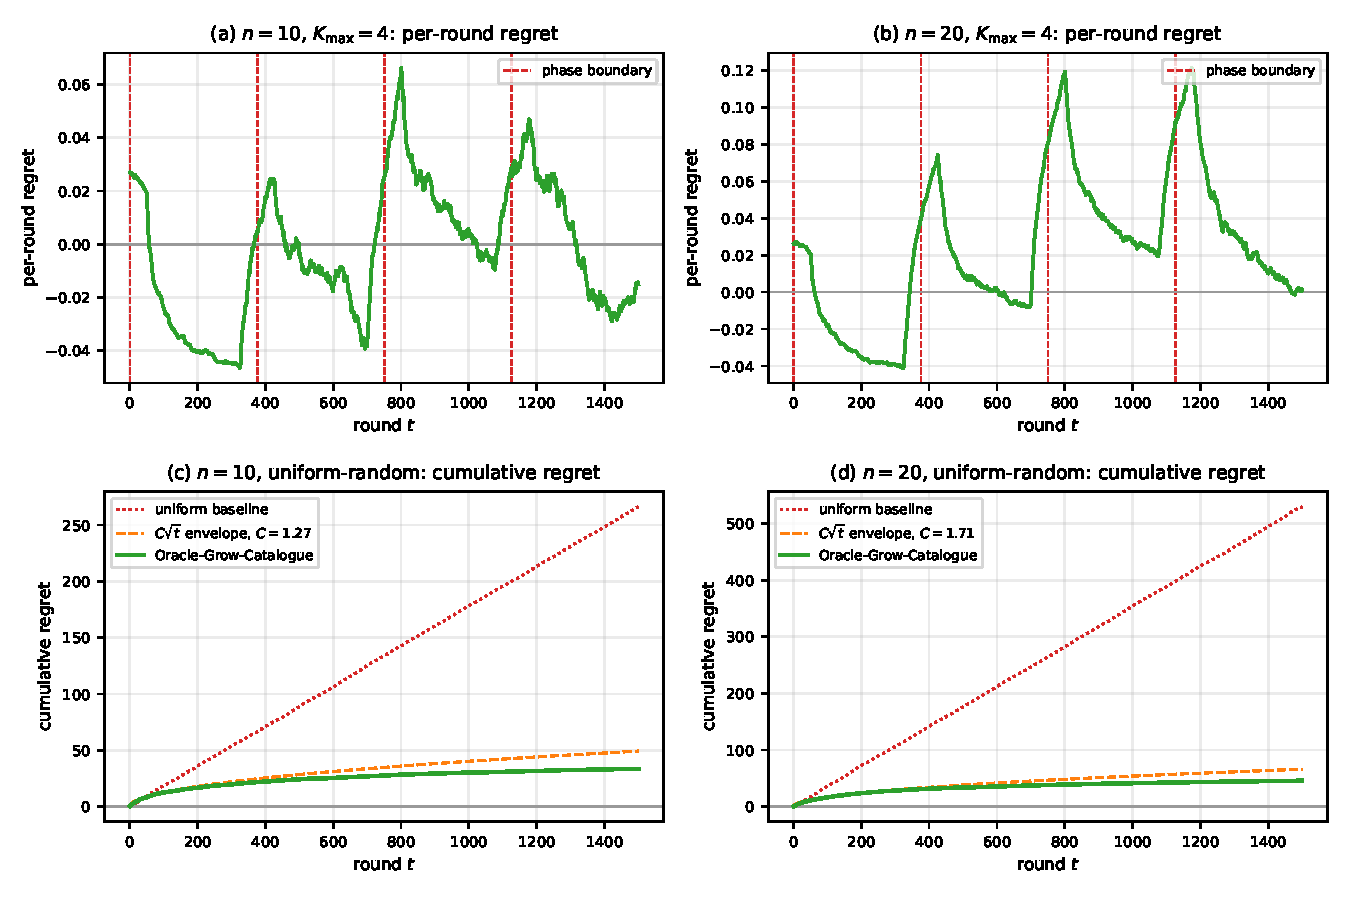
\includegraphics[width=0.96\textwidth]{figures/tractable_regret.pdf}
\vspace{-0.5em}
\caption{\Cref{alg:gc} with the oracle implementation of \Cref{sec:oracle},
$\Kmax=4$, $T=1500$, mean over $4$ seeds. (a), (b) per-round regret under the
staggered-uniform adversary, rolling window $101$; red dashed lines mark the
phase boundaries, at which a new type becomes available. (c), (d) cumulative regret under the uniform-random
adversary, against the $C\sqrt t$ envelope of \Cref{thm:main} and the uniform
baseline.}
\label{fig:tractable}
\end{figure*}

\subsection{Block revelation at $n=10$ and $n=20$}
\label{sec:exp-block}

\Cref{fig:block} runs \Cref{alg:bgc} under genuine partial-information
feedback: the simulator passes the algorithm the attacked target only, and at
the end of each revelation block calls it with the \emph{set} of types seen
so far and nothing else. The set is handed over as a list for convenience,
but the algorithm reads it only through membership tests, so neither the
order in which the types first attacked nor any frequency information can
leak through it. Panels (a) and (b) show cumulative regret against
the $Ct^{2/3}$ envelope of \Cref{thm:block} under the staggered-uniform
adversary, which is the interesting one here because it spreads the discovery
blocks across the horizon and so produces the $\Theta(\Kmax)$ epochs that
Step~8 of the proof pays for; the envelope constants are $C=1.72$ at $n=10$
and $C=1.25$ at $n=20$.

Panel (c) sweeps the revelation length $B$ over six doublings at fixed $T$.
The measured growth is linear in $B$, as \Cref{thm:block,thm:blocklb}
predict --- a least-squares fit over $B\in[4,256]$ has slope $0.47$ --- but
that slope is far below the worst-case $2K'=8$, and the panel draws both.
The gap is expected rather than a discrepancy: the worst case is attained
only by the nested adversary of \Cref{thm:blocklb}, which
\Cref{fig:impossible}(d) exhibits separately, and on a random instance most
of the rounds of a discovery block are not in fact wasted, because a strategy
tuned to the types already in the catalogue is usually not terrible against a
new one.

Panel (d) compares the two feedback models as $T$ grows, on the stationary
uniform-random adversary for the reason given in \Cref{sec:exp-full}. Over
$T\in\{250,500,1000,2000\}$ the block-revelation regret grows with fitted
exponent $0.664$, which is $2/3$ to within the resolution of the experiment
and is exactly the exponent of \Cref{thm:block}; the full-information regret
grows with exponent $0.317$, comfortably inside the $1/2$ of \Cref{thm:main}.
The asymmetry is not an accident of the instances. \Cref{alg:bgc} pays a
floor of $|C|$ exploration rounds in every estimation block whatever the
sequence does, so its $T^{2/3}$ is visible even on an easy sequence, whereas
\Cref{alg:gc} has no such floor and, as already observed in \Cref{sec:exp},
runs well inside its worst case against a stochastic adversary.

One implementation choice is worth stating, because it is where asymptotics
and simulation disagree. \Citet[Algorithm 1]{balcan2015} uses
$Z=n\bigl(T^{2}\log(n|C|)\bigr)^{1/3}$ estimation blocks, i.e.\ blocks of
$T/Z=T^{1/3}/\bigl(n\log^{1/3}(n|C|)\bigr)$ rounds, which at $n=10$, $|C|=4$
and $T=2000$ is less than one round --- fewer, certainly, than the $|C|=4$
exploration rounds a block must hold, since the tuning of \citet[Theorem
6.1]{balcan2015} is asymptotic. We therefore use blocks of
$\max\{|C|+1,\lceil T^{1/3}\rceil\}$ rounds, which has the same order in
$T$. At $T=2000$ and $\Kmax=4$ that is $13$ rounds, of which $4$ are spent
exploring, so roughly $31\%$ of all rounds are exploration; this is the main
reason the measured regret in panels (a) and (b) is an order of magnitude
above the full-information regret of \Cref{fig:tractable} at the same
horizon, and it is a constant-factor effect, not a change of exponent.

\begin{figure*}[t]
\centering
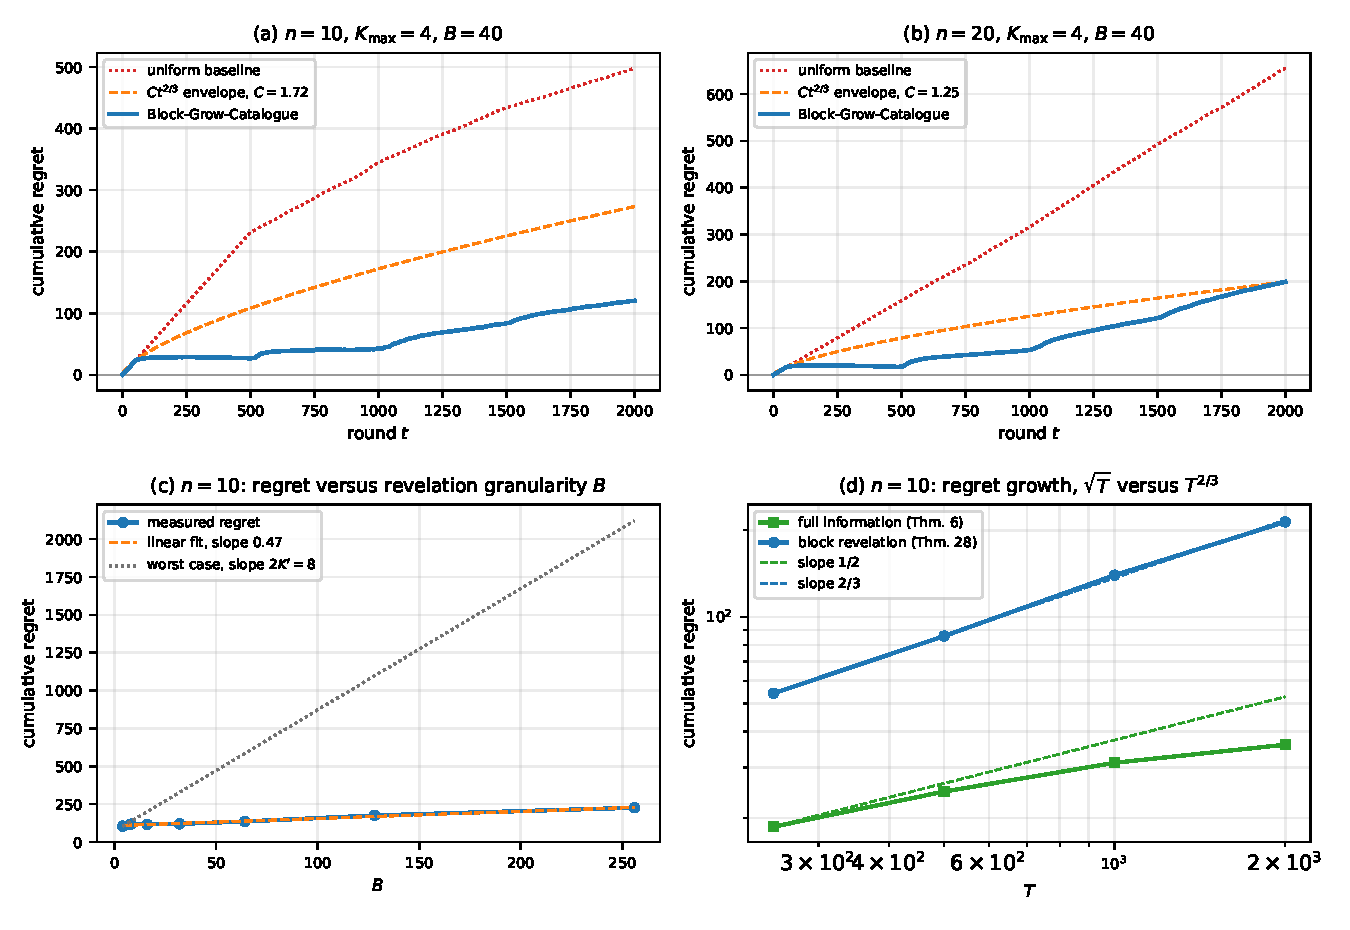
\includegraphics[width=0.96\textwidth]{figures/block_revelation.pdf}
\vspace{-0.5em}
\caption{\Cref{alg:bgc} under partial-information feedback with block
revelation, $\Kmax=4$, $T=2000$, mean over $4$ seeds. (a)--(c)
staggered-uniform adversary; (d) uniform-random adversary. (a), (b)
cumulative regret against the $Ct^{2/3}$ envelope of \Cref{thm:block}.
(c) final regret as a function of the revelation length $B$, against a
least-squares fit and against the worst-case slope $2K'$ of
\Cref{thm:block}. (d) full information (\Cref{thm:main}) against block
revelation (\Cref{thm:block}) as $T$ grows; fitted exponents $0.317$ and
$0.664$.}
\label{fig:block}
\end{figure*}

\subsection{The lower bounds, in simulation}
\label{sec:exp-imp}

\Cref{fig:impossible} plays the gadget $G_3$ of \Cref{sec:gadget} for real:
attacker types are built from the utility vectors of \Cref{eq:type-utils},
best responses are computed from those utilities, and the defender's payoff
is read off the attacked target. The defender is the optimal one for this
game, namely the midpoint version-space search of \Cref{thm:bits}(ii),
and the expectation over the hidden type is computed exactly, by averaging
over all $M$ candidates rather than by sampling.

Panel (a) is \Cref{thm:impossible}: with $M=2^{T}$ the measured expected
regret equals $T-2+(T+2)2^{-T}$ for every $T\le 14$, to machine precision,
confirming both the lower bound and the claim in \Cref{rem:tight-lb} that it
is exactly attained.

Panel (b) is \Cref{thm:bits}. The universe is fixed at $M=2^{10}$ and the
defender is helped by an oracle of budget $b\in\{0,2,4,6\}$ that names the
block of $M/2^{b}$ indices containing the true type, exactly as in the proof
of \Cref{thm:bits}(ii); everything else is the real game. Each curve
saturates, and it saturates at $\log_2 M-b-2$, which is the lower bound of
\Cref{thm:bits}(i): the measured values at $T=14$ are $8.01$, $6.04$, $4.13$
and $2.38$ against predictions $8$, $6$, $4$ and $2$. The hollow markers are
a separate run with budget $0$ on the smaller universe $\Univ_{M/2^{b}}$, and
they land on the corresponding curve to machine precision --- the regret
depends on $M$ and $b$ only through $\log_2 M-b$, which is what makes
\Cref{thm:bits} an accounting identity rather than two unrelated bounds. The
case $b=0$ also says that the linear growth in panel~(a) is caused by the
universe being infinite and by nothing else.

Panel (c) is \Cref{prop:sqrtT}, and it is the one panel that shows a
$T$-dependence rather than a saturation. With $|K|=2$ on the two-element
universe, follow the leader has measured regret $1.57$, $6.35$ and $25.60$ at
$T=16$, $256$ and $4096$, against the exact optimum
$\tfrac12\EE|N_1-N_2|=1.571$, $6.377$, $25.531$ and the floor
$\tfrac12\sqrt{\lfloor T/2\rfloor}=1.41$, $5.66$, $22.63$. The dotted line is
the same universe with $|K|=1$, where the regret is $0.5$ at every horizon.
The two curves are the phase transition of \Cref{rem:phase}.

Panel (d) is \Cref{thm:blocklb}: on the nested-interval instance the measured
regret tracks $|K|(B-2)$ across $|K|\in\{1,2,3,4\}$ and
$B\in\{4,8,16,32\}$, so the additive $\Theta(\Kmax B)$ of \Cref{thm:block} is
real and not an artefact of the analysis.

Panel (e) is \Cref{prop:adaptive}, on the same instances as panel (d) with
$|K|=4$ and $T=|K|B$, so that the two schemes are compared at the same
report budget $N=|K|=4$. Scheduling the four reports on a fixed grid costs
$|K|(B-2)$, which is $120$ rounds at $B=32$; letting the defender choose
their times costs exactly $4$, and the measured query count is $4.00$, so the
defender does not even exceed its budget. The measured adaptive regret is
$3.72$, $3.98$, $4.00$, $4.00$ for $B=4,8,16,32$ --- it is below $|K|$ only
because a lucky initial play occasionally hits the first type outright.

\begin{figure*}[t]
\centering
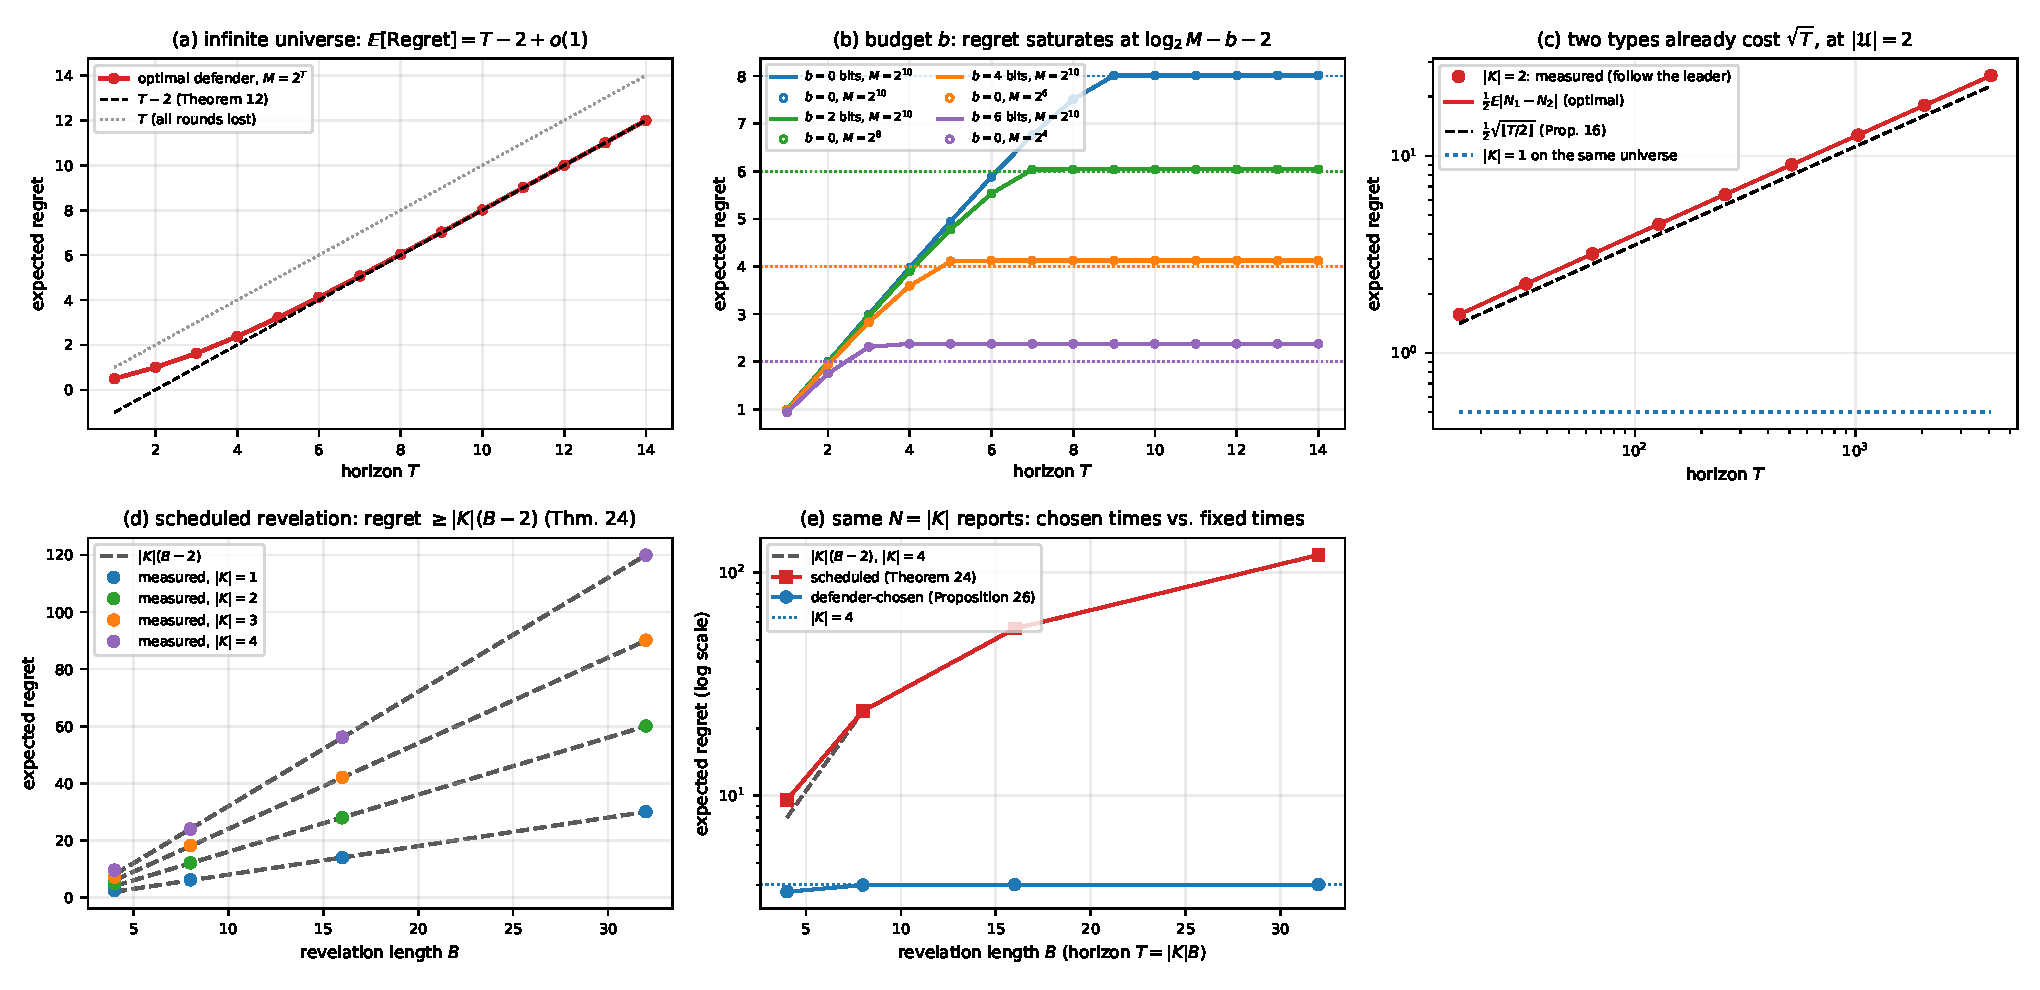
\includegraphics[width=0.96\textwidth]{figures/impossibility.pdf}
\vspace{-0.5em}
\caption{The gadget $G_3$ in simulation, against the optimal defender.
(a) \Cref{thm:impossible}: with $|\Univ_M|=2^{T}$ the regret is $T-2+o(1)$.
(b) \Cref{thm:bits}: with a budget of $b$ bits on a universe of resolution
$M=2^{10}$ the regret saturates at $\log_2 M-b-2$ (dotted lines), and a
budget-$b$ run on $\Univ_M$ (solid) coincides with a budget-$0$ run on
$\Univ_{M/2^{b}}$ (hollow markers). (c) \Cref{prop:sqrtT}: two types on a
two-element universe cost $\Theta(\sqrt T)$, one type costs $0.5$ at every
horizon. (d) \Cref{thm:blocklb}: on the nested
instance the regret matches $|K|(B-2)$ (dashed lines). (e)
\Cref{prop:adaptive}: the same $N=|K|$ reports cost $|K|(B-2)$ on a fixed
schedule and $|K|$ when the defender picks their times. Panels (c) and (e)
have logarithmic vertical axes.}
\label{fig:impossible}
\end{figure*}

% ==========================================================================
\section{Discussion and Open Problems}
\label{sec:conc2}

\Cref{sec:partial,sec:block} locate the boundary of learnability for the
unknown-$K$ repeated security game. On one side, \Cref{thm:main} shows that
an unknown attacker set of bounded size costs only a factor $\sqrt{\Kmax}$ as
long as the defender is told, after each round, which type attacked. On the
other side, \Cref{thm:impossible} shows that if the defender is told nothing
but the attacked target, then every algorithm loses all but two of the $T$
rounds --- not because the adversary has many types, but because the defender
cannot name the one type it faces. \Cref{thm:bits} quantifies
this exactly, and in a currency that a security operations centre can price:
on a universe of resolution $M$, and given \emph{any} side channel that emits
$b$ bits over the whole horizon, the optimal regret is
$\min\{T,\log_2 M-b\}\pm 3$. The attainable regret is the number of bits
still needed to name the attacker; it is linear precisely when that number
exceeds the horizon, and on an infinite universe no finite budget reduces it
at all.

Between the two lies \Cref{prob:block}, in which an oracle periodically
reports the \emph{set} of types encountered so far. The information it
supplies is exactly a list of names; it says nothing about when or how often
any of them attacked. \Cref{thm:block} shows that this is enough:
\Cref{alg:bgc} attains
$O(n\Kmax^{4/3}T^{2/3}\log^{1/3}(n\Kmax)+\Kmax B)$, the
partial-information rate of \citet[Theorem 6.1]{balcan2015} degraded by a
factor $\Kmax^{1/3}$ for the unknown catalogue and by an additive $\Kmax B$
for the batching, and \Cref{thm:blocklb} shows the additive term is tight up
to a factor $2B/(B-2)$, hence up to $2+o(1)$ once $B$ is large. \Cref{cor:B} turns this into a deployment statement: the
threat-intelligence report needs to arrive only $\tilde O(T^{1/3})$ times
over a horizon of length $T$ for the batching to be free --- and, by the
lower bound in the same corollary, not fewer.

Two views of the same picture from the online-learning literature are worth
recording, because they say where these results sit. The query-budget
statement of \Cref{thm:bits} is a security-game analogue of \emph{label
efficient prediction} \citep{cesabianchi2005}, where a learner may see the
loss vector on only a bounded number of rounds; the difference is that there
the budget limits how \emph{often} the learner may look, whereas
\Cref{def:budget} limits how \emph{much} it may be told in total, and
consequently the rate here is governed by $\log_2|\Univ|$ rather than by the
number of experts. The additive $\Theta(\Kmax B)$ of \Cref{thm:block,thm:blocklb}
is a delay phenomenon of the kind studied for general online learning under
delayed feedback \citep{joulani2013}; what is specific to the present setting
is that the delay applies not to the loss but to the \emph{identity} of the
opponent, and that \Cref{thm:impossible} makes the undelayed identity
indispensable rather than merely helpful.

Two independent obstructions are thus isolated. \Cref{thm:bits} is about
\emph{volume}: too few bits, and the type cannot be named. \Cref{thm:blocklb}
is about \emph{latency}: even an unrestricted number of bits, delivered on a
calendar of period $B$, still costs $\Theta(\Kmax B)$, because the defender
must play blind between the arrival of a type and the arrival of the report
that names it. \Cref{prop:adaptive} shows the two are genuinely different
resources: in $G_3$, letting the defender choose \emph{when} the same
$\Kmax$ reports arrive collapses the latency cost from $T-2\Kmax$ to
$\Kmax$.

Five questions are left open.

\paragraph{Is the exponent $2/3$ necessary here?}
\Cref{rem:price} observes that the exponent in \Cref{thm:block} is inherited
from \citet[Theorem 6.1]{balcan2015} and is untouched by the unknown
catalogue, so any improvement would improve their result. It is not known
whether $T^{2/3}$ is optimal for partial-information feedback even with $K$
known; the natural attack is to replace their explore-then-exploit estimator
by importance-weighted estimates on the exploit rounds, which would require a
version of \Cref{lem:contain} for a continuously updated estimator.

\paragraph{Is the factor $\Kmax^{1/3}$ necessary?}
It arises from H\"older over the at most $\Kmax$ epochs (Step~8), exactly as
the $\sqrt{\Kmax}$ of \Cref{thm:main} arises from Cauchy--Schwarz (Step~9 of
\Cref{sec:proof}). \Cref{thm:blocklb} lower bounds only the additive term, and
\Cref{prop:sqrtT} lower bounds only the $T$-dependence. A
lower bound of the form $\Omega(\Kmax^{c}T^{2/3})$ for some $c>0$, matching
the multiplicative price of not knowing $K$, is open in both the
full-information and the partial-information settings. The obvious attempt
--- running $\Kmax/2$ disjoint copies of the two-type construction of
\Cref{prop:sqrtT}, one per epoch --- does not work, and the reason is
instructive. Per-epoch lower bounds do not add, because the benchmark
\Cref{eq:pstar} is a \emph{single} fixed coverage vector: in $G_3$ with all
the intervals disjoint, \Cref{lem:hit} says that no $\pvec$ hits more than
one type at all, so the global benchmark is far weaker than the sum of the
per-epoch benchmarks and the global regret is correspondingly smaller. A
matching lower bound will have to make the epochs share a good comparator,
as the nested family of \Cref{thm:blocklb} does, while still forcing fresh
learning in each of them.

The complementary attack is on the upper bound: avoid the restart, and both
factors disappear with it, since with no epochs there is neither a
Cauchy--Schwarz nor a H\"older step. Algorithms that track a \emph{growing}
expert set \citep{mourtada2017} do exactly that, and \Cref{sec:related}
already notes them as a drop-in replacement for the Polynomial-Weights
sub-routine of \Cref{alg:gc}. What the proofs above show is that replacing
the sub-routine is not by itself enough: Steps~4 and 5 of \Cref{sec:proof}
also use the epoch structure, to pass from the epoch-local optimum to the
global $\pvec^{*}$. Under partial information the difficulty is sharper
still. The estimator of \Cref{lem:lift}(ii) is defined relative to a fixed
catalogue --- its spanner $\Lambda$ and the ambient set $\mathcal{W}$ both
change when $C$ grows --- so the estimates produced before and after a
discovery block are not estimates of comparable quantities, and cannot be
handed to a single continuously running learner without a new argument.

\paragraph{Confounded search: $\Kmax\ge 2$ on a finite universe.}
\Cref{thm:bits} pins the optimal regret on a resolution-$M$ universe
to $\min\{T,\log_2 M-b\}\pm 3$ when $\Kmax=1$, because a miss then identifies
a half of the version space unambiguously. For $\Kmax\ge 2$ the defender
does not know which of its opponents produced the observation, so the same
search is corrupted. \Cref{prop:sqrtT} settles one half of the question ---
the answer must contain an $\Omega(\sqrt{T})$ term, already at $M=2$ --- and
\Cref{rem:phase} records the two upper bounds we can write down,
$O(\sqrt{T\Kmax(n^2+\Kmax\log n)})$ under full information and
$O(T^{2/3}nM\log^{1/3}(nM))$ under partial information. Neither has any
$\log M$ in it, and the lower bound has no $M$ in it either, so the joint
dependence on $M$ and $\Kmax$ is entirely open. Note that
\Cref{thm:impossible} does not settle it: it shows the $M\to\infty$ limit is
$\Theta(T)$ for every $\Kmax\ge 1$, but says nothing about the finite-$M$
dependence for $\Kmax\ge 2$.

\paragraph{One theorem for volume and latency together.}
\Cref{thm:bits} charges an oracle for its bits and ignores their timing;
\Cref{thm:blocklb} charges for the timing and lets the bits be free. Neither
subsumes the other, and a defender buying threat intelligence pays for both
at once. The missing statement is a lower bound in terms of a pair
$(b,\lambda)$ --- total budget and worst-case delay between a type's first
attack and the first message that names it --- which should degrade to
\Cref{thm:bits} at $\lambda=0$ and to \Cref{thm:blocklb} at $b=\infty$. We
expect the right form to be
$\Omega\bigl(\min\{T,\log_2 M-b\}+\Kmax\lambda\bigr)$, but the two arguments
resist being run simultaneously: \Cref{lem:count} conditions on a transcript
that the latency argument needs to keep random. A related gap is the oracle
whose messages are unbounded in length but weak in content --- one that
reports the utilities of a uniformly random element of $D_\nu$, say. Such an
oracle is not covered by \Cref{thm:bits}, whose budget is a bound on message
\emph{length}, and the version-space construction of \Cref{thm:bits}(ii) does
not apply to it either.

\paragraph{Self-timed reports in a general game.}
\Cref{prop:adaptive} shows that in $G_3$ a defender that chooses its own
report times pays $\Kmax$ rather than $\Kmax B$, because there a missed round
is a certificate that the catalogue is stale. \Cref{rem:adaptive} explains
why the certificate is special to that gadget. Whether some other trigger ---
a statistical test on the estimator of \Cref{lem:lift}(ii), say --- recovers
a comparable saving in a general repeated SSG, and whether the $\Theta(\Kmax
T/N)$ of \Cref{cor:B} is the truth for self-timed queries, we leave open.
This is the question with the most direct operational content: it asks
whether it is better to subscribe to a periodic feed or to keep a budget of
on-demand lookups.


\bibliography{refs}




\end{document}
